\PassOptionsToPackage{quiet}{fontspec}
\documentclass{article}


%%%%%%%%%%%%%%%%%%% usepackage %%%%%%%%%%%%%%%%%%%

\usepackage[a4paper, margin=1in]{geometry}
\usepackage{ctex}

\usepackage{amsthm, amsfonts, amsmath, amssymb}
\usepackage{mathtools}
\usepackage{centernot}
\usepackage{arydshln}
\setcounter{MaxMatrixCols}{11}

\usepackage{booktabs}
\usepackage{graphicx}
\usepackage{setspace}
\usepackage[hidelinks]{hyperref}
\usepackage{framed}
\usepackage{float}

\usepackage{tcolorbox}
\tcbuselibrary{breakable}

\usepackage{xcolor}
\usepackage{multicol}
\usepackage{multirow}

\usepackage{enumitem}
\setlist{noitemsep}


%%%%%%%%%%%%%%%%%%%%%% math %%%%%%%%%%%%%%%%%%%%%%

\theoremstyle{definition}
\newtheorem{theorem}{定理}[section]
\newtheorem{corollary}[theorem]{推论}
\newtheorem{lemma}[theorem]{引理}
\newtheorem*{property}{性质}

\theoremstyle{definition}
\newtheorem{definition}{定义}[section]
\newtheorem{example}{例}[section]
\newtheorem{exercise}{练习}

\theoremstyle{remark}
\newtheorem*{remark}{注解}
\newtheorem*{note}{注意}
\newtheorem*{com}{注释}

\tcolorboxenvironment{example}{colback=blue!5!white, boxrule=0.5pt, breakable}
\tcolorboxenvironment{remark}{colback=green!10!white, boxrule=0.5pt, breakable}
\tcolorboxenvironment{note}{colback=yellow!10!white, boxrule=0.5pt, breakable}
\tcolorboxenvironment{proof}{colback=black!5!white, boxrule=0.5pt, breakable}


%%%%%%%%%%%%%%%%%% new command %%%%%%%%%%%%%%%%%%%
\newcommand{\ind}{\mathrel{\perp\!\!\!\!\perp}}
\newcommand{\Cov}{\mathrm{Cov}}
\newcommand{\Var}{\mathrm{Var}}
\newcommand{\E}{\mathbb{E}}
\newcommand{\G}{\mathbb{G}}
\newcommand{\V}{\mathbb{V}}
\newcommand{\Pb}{\mathbb{P}}
\newcommand{\sigmaXX}{\sigma_{\scalebox{.6}{$XX$}}}
\newcommand{\sigmaYY}{\sigma_{\scalebox{.6}{$YY$}}}
\newcommand{\sigmaXY}{\sigma_{\scalebox{.6}{$XY$}}}
\newcommand{\sigmaYX}{\sigma_{\scalebox{.6}{$YX$}}}
\newcommand{\sigmaXYZ}{\sigma_{\scalebox{.6}{$XY\vert Z$}}}
\newcommand{\sigmaYXZ}{\sigma_{\scalebox{.6}{$YX\vert Z$}}}
\newcommand{\pa}{\mathrm{pa}}
\newcommand{\ch}{\mathrm{ch}}
\newcommand{\nb}{\mathrm{nb}}
\newcommand{\bd}{\mathrm{bd}}
\newcommand{\cl}{\mathrm{cl}}
\newcommand\norm[1]{\Vert#1\Vert}


%%%%%%%%%%%%%%%%%%%%%% main %%%%%%%%%%%%%%%%%%%%%%

\begin{document}
% \begin{sloppypar}

\title{课程笔记·UCAS矩阵论}
\author{xyfJASON\\中国科学院大学}
\date{}

\maketitle
\tableofcontents
\pagebreak

\section{样本空间与概率}

\subsection{概率模型}

\begin{definition}[概率模型的基本构成]
概率模型由样本空间和概率律构成:
\begin{itemize}
    \item 样本空间 $\Omega$:一个试验的所有可能结果的集合。
    \item 概率律:为试验结果的集合 $A$(称为事件)确定一个非负数 $\Pb(A)$,称为事件 $A$ 的概率。概率律需要满足概率公理。
\end{itemize}
\begin{figure}[H]
    \centering
    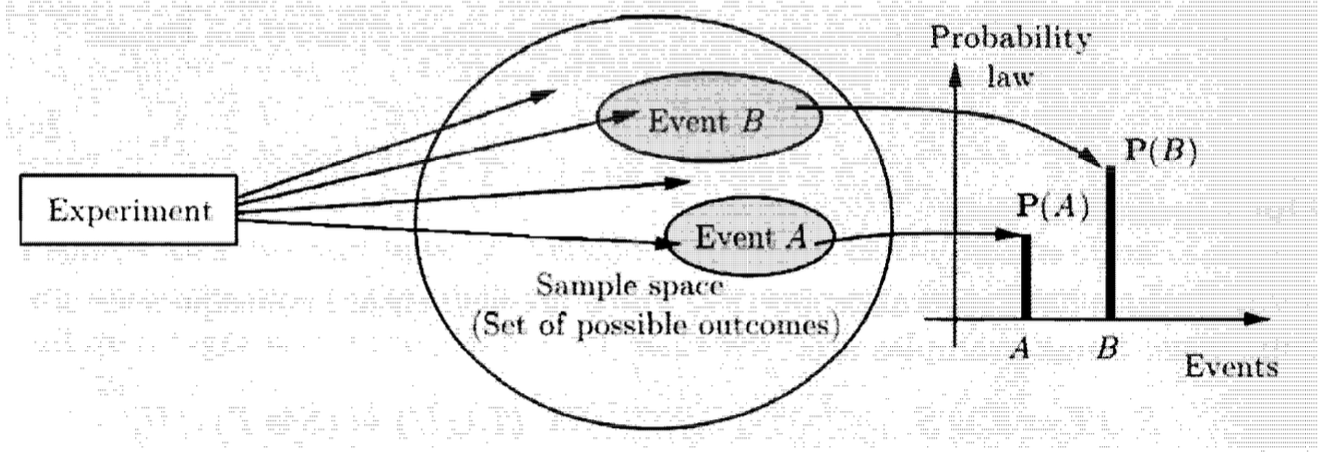
\includegraphics[width=0.8\linewidth]{figs/概率模型的基本构成.png}
    \caption{概率模型的基本构成}
    \label{fig:prob-model-components}
\end{figure}
\end{definition}

\begin{definition}[概率公理]
概率满足以下几条公理:
\begin{enumerate}
    \item 非负性:对一切事件 $A$,满足 $\Pb(A)\geq 0$.
    \item 归一化:整个样本空间为必然事件,即 $\Pb(\Omega)=1$.
    \item 可数可加性:设 $A_1,A_2,\ldots$ 是一列互不相容事件,则 $\Pb(A_1\cup A_2\cup\cdots)=\Pb(A_1)+\Pb(A_2)+\cdots$.
\end{enumerate}
\end{definition}

\begin{property}
设 $A,B,C$ 为事件,则由概率公理可以推导出如下性质:
\begin{itemize}
    \item 空事件概率为 0,即 $\Pb(\varnothing)=0$
    \item $A\subset B\implies \Pb(A)\leq \Pb(B)$
    \item $\Pb(A\cup B)=\Pb(A)+\Pb(B)-\Pb(A\cap B)$
    \item $\Pb(A\cup B)\leq \Pb(A)+\Pb(B)$
    \item $\Pb(A\cup B\cup C)=\Pb(A)+\Pb(A^c\cap B)+\Pb(A^c\cap B^c\cap C)$
\end{itemize}
\end{property}


\subsection{条件概率}

\begin{definition}[条件概率]
设 $A,B$ 为两个事件且 $\Pb(B)>0$,定义 $B$ 发生的条件下 $A$ 发生的概率为:\[\Pb (A\vert B)=\frac{\Pb(A\cap B)}{\Pb(B)},\quad \Pb(B)>0\]
\end{definition}

\begin{theorem}
条件概率是一个公理化定义下的概率,从而概率的所有性质都适用于条件概率。
\end{theorem}
\begin{proof}
只需验证条件概率是否满足非负性、归一化和可数可加性即可。
\begin{enumerate}
    \item 非负性:显然;
    \item 归一化:\[\Pb(\Omega\vert B)=\frac{\Pb(\Omega\cap B)}{\Pb(B)}=\frac{\Pb(B)}{\Pb(B)}=1\]
    \item 可数可加性:
    \begin{align*}
    \Pb\left(\left.\bigcup_{i=1}^nA_i\right\vert B\right)&=\frac{\Pb\left(\left(\bigcup_{i=1}^nA_i\right)\cap B\right)}{\Pb(B)}=\frac{\Pb\left(\bigcup_{i=1}^n(A_i\cap B)\right)}{\Pb(B)}\\
    &=\frac{\sum_{i=1}^n\Pb(A_i\cap B)}{\Pb(B)}=\sum_{i=1}^n\Pb(A_i\vert B)
    \end{align*}
\end{enumerate}
\end{proof}

\begin{theorem}[乘法公式]
设 $A,B$ 为两个事件,则由定义易知:\[\Pb (A\cap B)=\Pb(B)\Pb(A\vert B)\]
\end{theorem}

\begin{corollary}
设 $A_1,A_2,\ldots,A_n$ 为 $n$ 个事件,则:\[\Pb(A_1A_2\cdots A_n)=\Pb(A_1)\Pb(A_2\vert A_1)\Pb(A_3\vert A_1A_2)\cdots\Pb(A_n\vert A_1A_2\cdots A_{n-1})\]
\end{corollary}


\subsection{全概率公式和贝叶斯公式}

\begin{theorem}[全概率公式]
设 $A_1,A_2,\cdots,A_n$ 互不相容,$B\subset A_1\cup A_2\cup\cdots\cup A_n$,则:\[\Pb(B)=\sum_{i=1}^n\Pb(A_i)\Pb(B\vert A_i)\]
\end{theorem}
\begin{proof}
\[\Pb(B)=\Pb\left(B\cap \left(\bigcup_{i=1}^nA_i\right)\right)=\Pb\left(\bigcup_{i=1}^n(A_i\cap B)\right)=\sum_{i=1}^n\Pb(A_i\cap B)=\sum_{i=1}^n\Pb(A_i)\Pb(B\vert A_i)\]
\end{proof}

\begin{theorem}[贝叶斯公式]
设 $A_1,A_2,\cdots,A_n$ 互不相容且 $\Pb(A_i)>0$,$B\subset A_1\cup A_2\cup\cdots\cup A_n$,则:
\[\Pb(A_i\vert B)=\frac{\Pb(A_i\cap B)}{\Pb(B)}=\frac{\Pb(A_i)\Pb(B\vert A_i)}{\sum\limits_{j=1}^n\Pb(A_j)\Pb(B\vert A_j)}\]
其中 $\Pb(A_i)$ 称作先验概率,$\Pb(A_i\vert B)$ 称作后验概率。
\end{theorem}

\begin{remark}[关于贝叶斯公式的理解]
视事件 $A_i$ 是导致事件 $B$ 发生的原因,我们对于事件 $A_i$ 已有一个先验概率 $\Pb(A_i)$,现在事件 $B$ 发生了,这必然给我们带了一定的信息,于是我们可以由此修正 $A_i$ 发生的概率,得到 $\Pb(A_i\vert B)$,即后验概率。
\end{remark}


\subsection{独立性}

\begin{definition}[独立]
设 $A,B$ 是两个事件,称 $A$ 与 $B$ 独立,若:\[\Pb(A\cap B)=\Pb(A)\Pb(B)\]
\end{definition}
\begin{com}
若 $\Pb(B)\neq 0$,则 $A$ 与 $B$ 独立等价于:
\[\Pb(A\vert B)=\Pb(A)\]
直观上,这说明事件 $B$ 的发生与否并不给 $A$ 带来信息,不改变 $A$ 发生的概率。
\end{com}
\begin{note}
事件的独立性常常不能直观地看出来。例如,若事件 $A$ 与事件 $B$ 互不相容,并且 $\Pb(A)>0,\,\Pb(B)>0$,则它们一定不独立,因为 $\Pb(A\cap B)=0\neq\Pb(A)\Pb(B)$. 直观上,事件 $B$ 发生意味着 $A$ 一定没有发生,因此 $B$ 的发生与否会给 $A$ 带来信息。
\end{note}

\begin{theorem}
设事件 $A$ 与事件 $B$ 独立,则 $A$ 与 $B^c$ 也独立。
\end{theorem}
\begin{proof}
由于 $A$ 可写作两个不相容事件之并 $A=(A\cap B)\cup (A\cap B^c)$,故:
\[
\Pb(A)=\Pb(A\cap B)+\Pb(A\cap B^c)
\]
于是:
\[
\Pb(A\cap B^c)=\Pb(A)-\Pb(A\cap B)=\Pb(A)-\Pb(A)\Pb(B)=\Pb(A)(1-\Pb(B))=\Pb(A)\Pb(B^c)
\]
\end{proof}

\begin{definition}[条件独立]
给定事件 $C$,称事件 $A,B$ 在给定 $C$ 下条件独立,若:
\[\Pb(A\cap B\vert C)=\Pb(A\vert C)\Pb(B\vert C)\]
\end{definition}
\begin{com}
$A,B$ 条件独立并不能推出 $A,B$ 独立,反之亦不成立。
\end{com}

\begin{definition}[一组事件的相互独立性]
设 $A_1,A_2,\ldots,A_n$ 是一组事件,称它们相互独立,若:
\[
\Pb\left(\bigcap_{i\in S}A_i\right)=\prod_{i\in S}\Pb(A_i),\quad\forall S\subset\{1,2,\ldots,n\}
\]
\end{definition}
\begin{note}[两两独立与相互独立]
设 $A_1,A_2,A_3$ 相互独立,则有:
\begin{gather*}
\Pb(A_1\cap A_2)=\Pb(A_1)\Pb(A_2)\\
\Pb(A_2\cap A_3)=\Pb(A_1)\Pb(A_3)\\
\Pb(A_1\cap A_3)=\Pb(A_1)\Pb(A_3)\\
\Pb(A_1\cap A_2\cap A_3)=\Pb(A_1)\Pb(A_2)\Pb(A_3)
\end{gather*}
前三个式子称作两两独立。但是第四个式子也非常重要,它并不是前三个式子的推论;反之,第四个式子也不能推出前三个式子。
\end{note}
\begin{example}[两两独立不能推出独立]
设试验是抛掷两枚均匀的硬币,考虑事件:
\[H_1=\{\text{第一次正面}\},\quad H_2=\{\text{第二次正面}\},\quad D=\{\text{两次结果不同}\}\]
则易知 $H_1$ 与 $H_2$ 独立。另外,
\[
\Pb(D\vert H_1)=\frac{\Pb(D\cap H_1)}{\Pb(H_1)}=\frac{1/4}{1/2}=\frac{1}{2}=\Pb(D)
\]
故 $D$ 与 $H_1$ 独立。同理可知 $D$ 与 $H_2$ 独立,故 $H_1,H_2,D$ 两两独立。但是:
\[
\Pb(H_1\cap H_2\cap D)=0\neq \Pb(H_1)\Pb(H_2)\Pb(D)=\frac{1}{2}\cdot\frac{1}{2}\cdot\frac{1}{2}
\]
故 $H_1,H_2,D$ 不是独立的。
\end{example}
 \pagebreak
\section{随机变量}

\subsection{基本概念}

\begin{definition}[随机变量]
随机变量是试验结果的实值函数。
\begin{figure}[H]
    \centering
    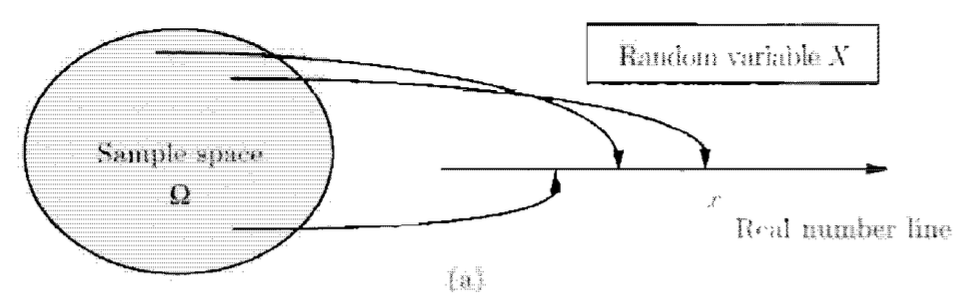
\includegraphics[width=0.65\linewidth]{figs/随机变量示意图.png}
    \caption{随机变量示意图}
    \label{fig:random-variable}
\end{figure}
\end{definition}
\begin{com}
一般用大写字母表示随机变量,小写字母表示其取值。
\end{com}

\begin{definition}[离散随机变量]
若一个随机变量的值域为有限集或可数集,则称这个随机变量是离散的。
\end{definition}

\begin{definition}[概率质量函数]
定义随机变量 $X$ 取值为 $x$ 的概率为事件 $\{X=x\}$ 的概率,即所有与 $x$ 对应的试验结果组成的事件的概率,记作 $p_X(x)$,即:
\[p_X(x)=\Pb(\{X=x\})\]
称 $p_X$ 为 $X$ 的概率质量函数 (PMF).
\end{definition}

\begin{property}
PMF 满足非负性和归一化条件:
\[\sum_x p_X(x)=\sum_x\Pb(X=x)=1\]
\end{property}
\begin{property}
设 $S$ 为任一 $X$ 可能取值的集合,则:
\[\Pb(X\in S)=\sum_{x\in S}p_X(x)\]
\end{property}

\begin{example}
常见的离散随机变量包括伯努利、二项、几何和泊松随机变量等,详见附录 \ref{sec:random-variables}.
\end{example}

\begin{definition}[连续随机变量,概率密度函数]
对随机变量 $X$,若存在一个非负函数 $f_X$,使得:
\[
\Pb(X\in B)=\int_Bf_X(x)\mathrm dx
\]
对实数轴的集合 $B$ 都成立\footnote{本书只考虑黎曼积分,且 $f_X$ 为有有限/可数个间断点的分段连续函数。},则称 $X$ 为连续的随机变量,函数 $f_X$ 称为概率密度函数 (PDF). 特别地,当 $B$ 是一个区间时,有:
\[
\Pb(a\leq X\leq b)=\int_a^bf_X(x)\mathrm dx
\]
\end{definition}
\begin{property}
PDF 满足非负性和归一化条件:
\[\int_{-\infty}^{\infty}f_X(x)\mathrm dx=\Pb(-\infty<X<\infty)=1\]
\end{property}
\begin{property}
对于充分小的 $\delta$,有:
\[\Pb(x\leq X\leq x+\delta)=\int_x^{x+\delta}f_X(x)\mathrm dx\approx f(x)\cdot\delta\]
\end{property}

\begin{example}
常见的连续随机变量包括均匀、指数和正态随机变量等,详见附录 \ref{sec:random-variables}.
\end{example}


\subsection{分布函数}

\begin{definition}[分布函数]
设 $X$ 是一个随机变量(离散或连续),定义其分布函数(CDF)$F_X$ 为:
\[
F_X(x)=\Pb(X\leq x)=\begin{dcases}
    \sum_{k\leq x}p_X(k),&\text{$X$ 离散}\\
    \int_{-\infty}^xf_X(t)\mathrm dt,&\text{$X$ 连续}
\end{dcases}
\]
\end{definition}
\begin{com}
分布函数统一刻画了离散和连续情形。离散情形下的 PMF、连续情形下的 PDF 和一般情形下的 CDF 都是相应随机变量的概率律。
\end{com}

\begin{property}
设 $F_X$ 是随机变量 $X$ 的分布函数,则:
\begin{itemize}
    \item $F_X$ 单调非减。
    \item $F_X(x)\to 0\;(x\to-\infty),;F_X(x)\to1(x\to\infty)$.
    \item 当 $X$ 是离散随机变量时,$F_X$ 是阶梯函数。
    \item 当 $X$ 是连续随机变量时,$F_X$ 是连续函数。
\end{itemize}
\end{property}

\begin{theorem}[分布列与分布函数]
设 $X$ 是离散随机变量且取整数值,则:
\[
F_X(k)=\sum_{i=-\infty}^kp_X(i),\quad p_X(k)=F_X(k)-F_X(k-1)
\]
\end{theorem}
\begin{theorem}[概率密度函数与分布函数]
设 $X$ 是连续随机变量,则:
\[
F_X(x)=\int_{-\infty}^xf_X(t)\mathrm dt,\quad f_X(x)=\frac{\mathrm d}{\mathrm dx}F_X(x)
\]
第二个等式只在分布函数可微处成立。
\end{theorem}


\subsection{期望和方差}

\begin{definition}[期望/均值]
随机变量 $X$ 的期望定义为:
\[
\E X=\begin{dcases}
    \sum_x xp_X(x),&\text{$X$ 离散}\\
    \int_{-\infty}^{\infty}xf_X(x)\mathrm dx,&\text{$X$ 连续}
\end{dcases}
\]
特别地,对于连续情形,若 $f_X$ 不是绝对可积的,即 $\int_{-\infty}^\infty |x|f_X(x)\mathrm dx=\infty$,则称期望不存在。
\end{definition}

\begin{definition}[矩,中心矩]
定义随机变量 $X$ 的 $n$ 阶矩为 $\E[X^n]$,$n$ 阶中心矩为 $\E[(X-\E X)^n]$.
\end{definition}

\begin{definition}[方差,标准差]
定义随机变量 $X$ 的方差为其 2 阶中心矩,标准差为方差的平方根:
\[
\var(X)=\E\left[(X-\E X)^2\right],\quad \sigma(X)=\sqrt{\var(X)}
\]
\end{definition}

\begin{theorem}[随机变量函数的期望]
设 $X$ 是一随机变量,则 $Y=g(X)$ 的期望为:
\[\E Y=\E[g(X)]=\begin{dcases}
    \sum_xg(x)p_X(x),&\text{$X$ 离散}\\
    \int_{-\infty}^{+\infty}g(x)f_X(x)\mathrm dx,&\text{$X$ 连续}
\end{dcases}
\]
因此,我们不必先求出 $Y$ 的分布,只需知道 $X$ 的分布就能求出 $Y$ 的期望。
\end{theorem}

\begin{theorem}[随机变量的线性函数的期望和方差]
设 $X$ 是一个随机变量,$Y=aX+b$,其中 $a,b$ 为常数,则:
\[\E Y=a\E X+b,\quad \var(Y)=a^2\var(X)\]
\end{theorem}
\begin{proof}
仅对离散情形证明,连续情形类似。
\begin{gather*}
\E Y=\sum_x(ax+b)p_X(x)=a\sum_x xp_X(x)+b\sum_xp_X(x)=a\E X+b\\
\var(Y)=\E[(Y-\E Y)^2]=\E[((aX+b)-(a\E X+b))^2]=a^2\E[(X-\E X)^2]=a^2\var(X)
\end{gather*}
\end{proof}

\begin{theorem}[用矩表达方差]
设 $X$ 是一个随机变量,则:
\[
\var(X)=\E[X^2]-(\E X)^2
\]
\end{theorem}
\begin{proof}
\begin{align*}
\var(X)&=\E\left[(X-\E X)^2\right]\\
&=\E\left[X^2-2X\E X+(\E X)^2\right]\\
&=\E[X^2]-2 \E X\cdot \E X+(\E X)^2\\
&=\E[X^2]-(\E X)^2
\end{align*}
\end{proof}

\begin{example}
常见随机变量的期望和方差及其推导过程见附录 \ref{sec:random-variables}.
\end{example}


\subsection{联合分布与边缘分布}

\begin{figure}[H]
    \centering
    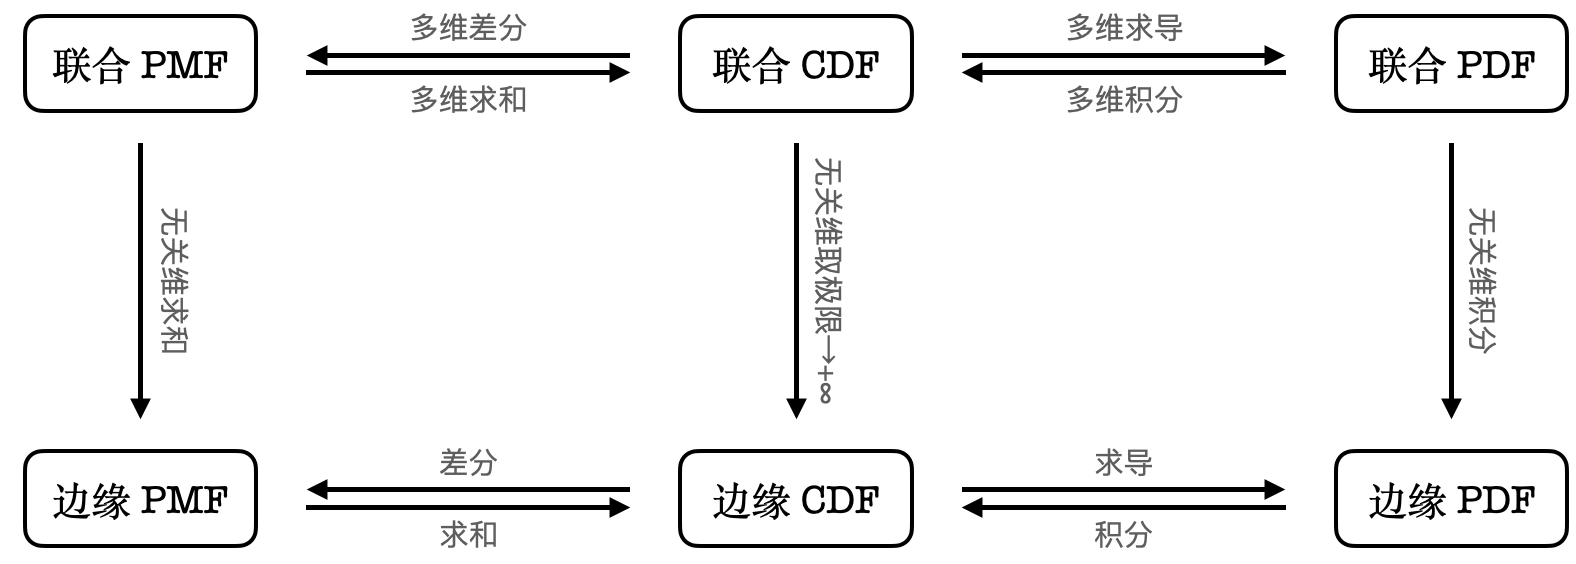
\includegraphics[width=0.8\linewidth]{figs/联合分布与边缘分布.png}
    \caption{联合分布与边缘分布的关系概览}
    \label{fig:union-marginal}
\end{figure}

\begin{definition}[联合概率质量函数]
设 $X,Y$ 是离散随机变量,定义 $(X,Y)$ 取值 $(x,y)$ 的概率为事件 $\{X=x,Y=y\}$ 的概率,记作 $p_{X,Y}(x,y)$,即:\[p_{X,Y}(x,y)=\Pb(X=x,Y=y)\]
称 $p_{X,Y}$ 为 $X,Y$ 的联合概率质量函数。
\end{definition}

\begin{definition}[联合概率密度函数]
设 $X,Y$ 是连续随机变量,若存在一个非负二元函数 $f_{X,Y}$ 使得:
\[
\Pb((X,Y)\in B)=\iint_{(x,y)\in B}f_{X,Y}(x,y)\mathrm dx\mathrm dy
\]
对平面上任意集合 $B$ 成立,则称 $f_{X,Y}$ 为联合概率密度函数。特别地,当 $B$ 是一个矩形区域时有:
\[
\Pb(a\leq X\leq b,c\leq Y\leq d)=\int_c^d\int_a^b f_{X,Y}(x,y)\mathrm dx\mathrm dy
\]
\end{definition}

\begin{property}
联合 PDF 满足归一化条件:
\[\int_{-\infty}^{\infty}\int_{-\infty}^{\infty}f_{X,Y}(x,y)\mathrm dx\mathrm dy=1\]
\end{property}
\begin{property}
对于充分小的 $\delta$,有:
\[\Pb(a\leq X\leq a+\delta,c\leq Y\leq c+\delta)=\int_c^{c+\delta}\int_a^{a+\delta}f_{X,Y}(x,y)\mathrm dx\mathrm dy\approx f_{X,Y}(a,c)\cdot\delta^2\]
\end{property}

\begin{theorem}[边缘概率质量函数]
设 $X,Y$ 是离散随机变量且联合 PMF 为 $p_{X,Y}$,则:
\[
p_X(x)=\sum_y p_{X,Y}(x,y),\quad p_Y(y)=\sum_xp_{X,Y}(x)
\]
称 $p_X$ 和 $p_Y$ 为边缘概率质量函数。
\end{theorem}

\begin{theorem}[边缘概率密度函数]
设 $X,Y$ 是连续随机变量且联合 PDF 为 $f_{X,Y}$,则:
\[
f_X(x)=\int_{-\infty}^{\infty}f_{X,Y}(x,y)\mathrm dy,\quad f_Y(y)=\int_{-\infty}^{\infty}p_{X,Y}(x)\mathrm dx
\]
称 $f_X$ 和 $f_Y$ 为边缘概率密度函数。
\end{theorem}

\begin{definition}[联合分布函数]
设 $X,Y$ 是两个随机变量(离散或连续),定义其联合分布函数为:
\[
F_{X,Y}(x,y)=\Pb(X\leq x,Y\leq y)
\]
\end{definition}

\begin{theorem}[联合概率密度函数与联合分布函数]
若随机变量 $X,Y$ 有联合概率密度函数 $f_{X,Y}$,则:
\[
F_{X,Y}(x,y)=\int_{-\infty}^x\int_{-\infty}^yf_{X,Y}(s,t)\mathrm ds\mathrm dt,\quad f_{X,Y}(x,y)=\frac{\partial^2}{\partial x\partial y}F_{X,Y}(x,y)
\]
\end{theorem}

\begin{theorem}[随机变量的二元函数的期望]
设 $X$ 和 $Y$ 是随机变量,则 $Z=g(X,Y)$ 的期望为:
\[
\E Z=\E[g(X,Y)]=\begin{dcases}
    \sum_{x}\sum_{y}g(x,y)p_{X,Y}(x,y),&\text{$X,Y$ 离散}\\
    \int_{-\infty}^{\infty}\int_{-\infty}^{\infty}g(x,y)f_{X,Y}(x,y)\mathrm dx\mathrm dy,&\text{$X,Y$ 连续}
\end{dcases}
\]
\end{theorem}

\begin{theorem}[随机变量的二元线性函数的期望]
设 $X$ 和 $Y$ 是随机变量,$a,b,c$ 为常数,则:
\[
\E[aX+bY+c]=a\E X+b\E Y+c
\]
\end{theorem}

\begin{theorem}[随机变量的多元线性函数的期望]
设 $X_1,X_2,\ldots,X_n$ 是 $n$ 个随机变量,$a_1,a_2,\ldots,a_n$ 是 $n$ 个常数,则:
\[
\E[a_1X_1+a_2X_2+\cdots+a_nX_n]=a_1\E X_2+a_2\E X_2+\cdots+a_n\E X_n
\]
\end{theorem}


\subsection{条件}

\begin{definition}[条件分布]
设 $X,Y$ 是离散随机变量,定义给定 $Y=y$ 下 $X$ 的条件概率质量函数为:
\[
p_{X\vert Y}(x\vert y)=\Pb(X=x\vert Y=y)=\frac{\Pb(X=x,Y=y)}{\Pb(Y=y)}=\frac{p_{X,Y}(x,y)}{p_Y(y)}
\]
类似地,设 $X,Y$ 是连续随机变量,定义给定 $Y=y$ 下 $X$ 的条件概率密度函数为:
\[
f_{X\vert Y}(x\vert y)=\frac{f_{X,Y}(x,y)}{f_Y(y)}
\]
\end{definition}

\begin{property}
条件 PMF/PDF 满足归一化条件:
\begin{gather*}
\sum_x p_{X\vert Y}(x\vert y)=1,\quad\text{$X$ 离散}\\
\int_{-\infty}^{\infty}f_{X\vert Y}(x\vert y)\mathrm dx=1,\quad\text{$X$ 连续}
\end{gather*}
\end{property}

\begin{theorem}[条件分布与联合分布]
设 $X,Y$ 是随机变量,由定义可知:
\begin{gather*}
p_{X,Y}(x,y)=p_Y(y)p_{X\vert Y}(x\vert y)=p_X(x)p_{Y\vert X}(y\vert x),\quad\text{$X$ 离散}\\
f_{X,Y}(x,y)=f_Y(y)f_{X\vert Y}(x\vert y)=f_X(x)f_{Y\vert X}(y\vert x),\quad\text{$X$ 连续}
\end{gather*}
\end{theorem}

\begin{theorem}[条件分布与边缘分布]
设 $X,Y$ 是随机变量,则根据全概率公式,有:
\begin{gather*}
p_X(x)=\sum_y p_{X\vert Y}(x\vert y)p_Y(y),\quad\text{$X$ 离散}\\
f_X(x)=\int_{-\infty}^{\infty} f_{X\vert Y}(x\vert y)f_Y(y)\mathrm dy,\quad\text{$X$ 连续}
\end{gather*}
\end{theorem}

\begin{theorem}[贝叶斯公式]
设 $X,Y$ 是随机变量,则有:
\begin{gather*}
p_{X\vert Y}(x\vert y)=\frac{p_{X,Y}(x,y)}{p_Y(y)}=\frac{p_{Y\vert X}(y\vert x)p_X(x)}{\sum_x p_{Y\vert X}(y\vert x)p_X(x)},\quad\text{$X,Y$ 离散}\\
f_{X\vert Y}(x\vert y)=\frac{f_{X,Y}(x,y)}{f_Y(y)}=\frac{f_{Y\vert X}(y\vert x)f_X(x)}{\int_{-\infty}^{\infty}f_{Y\vert X}(y\vert x)f_X(x)\mathrm dx},\quad\text{$X,Y$ 连续}
\end{gather*}
\end{theorem}

\begin{definition}[条件期望]
设 $X,Y$ 是随机变量,则给定 $Y=y$ 下 $X$ 的条件期望为:
\[
\E[X\vert Y=y]=\begin{dcases}
    \sum_xxp_{X\vert Y}(x\vert y),&\text{$X$ 离散}\\
    \int_{-\infty}^{\infty}xf_{X\vert Y}(x\vert y)\mathrm dx,&\text{$X$ 连续}
\end{dcases}
\]
对于随机变量的函数 $g(X)$,有:
\[
\E[g(X)\vert Y=y]=\begin{dcases}
    \sum_xg(x)p_{X\vert Y}(x\vert y),&\text{$X$ 离散}\\
    \int_{-\infty}^{\infty}g(x)f_{X\vert Y}(x\vert y)\mathrm dx,&\text{$X$ 连续}
\end{dcases}
\]
\end{definition}

\begin{note}
$\E[X|Y=y]$ 是一个数,其值依赖于 $y$,因此 $\E[X|Y]$ 是关于随机变量 $Y$ 的函数,从而也是一个随机变量。
\end{note}

\begin{theorem}[全期望公式]
设 $X,Y$ 是随机变量(离散或连续)且 $X$ 期望存在,则:
\[
\E X=\E[\E[X\vert Y]]=\begin{dcases}
    \sum_y \E[X\vert Y=y]p_Y(y),&\text{$Y$ 离散}\\
    \int_{-\infty}^{\infty} \E[X\vert Y=y]f_Y(y)\mathrm dy,&\text{$Y$ 连续}
\end{dcases}
\]
\end{theorem}
\begin{proof}
仅对离散情形证明,连续情形类似。
\begin{align*}
\E X&=\sum_x xp_X(x)\\
&=\sum_x x\sum_yp_{X|Y}(x\vert y)p_Y(y)\\
&=\sum_yp_Y(y)\sum_xxp_{X|Y}(x\vert y)\\
&=\sum_y \E[X\vert Y=y]p_Y(y)
\end{align*}
其中第二行应用了全概率公式。
\end{proof}

\begin{remark}
全期望公式常常是“反过来”使用的:当 $\mathbb EX$ 不好计算时,引入 $Y$ 转而计算 $\mathbb E[\mathbb E[X\vert Y]]$.
\end{remark}

\begin{definition}[条件方差]
设 $X,Y$ 是随机变量,则给定 $Y=y$ 下 $X$ 的条件方差为:
\[
\var(X\vert Y=y)=\E[(X-\E[X\vert Y=y])^2\vert Y=y]
\]
\end{definition}

\begin{note}
$\var(X\vert Y=y)$ 是一个数,其值依赖于 $y$,因此 $\var(X\vert Y)$ 是关于随机变量 $Y$ 的函数,从而也是一个随机变量,并且有:
\[
\var(X\vert Y)=\E[(X-\E[X\vert Y])^2\vert Y]=\E[X^2\vert Y]-(\E[X\vert Y])^2
\]
\end{note}

\begin{theorem}[全方差公式]
设 $X,Y$ 是随机变量且 $X$ 方差存在,则:
\[
\var(X)=\E[\var(X\vert Y)]+\var(\E[X\vert Y])
\]
\end{theorem}
\begin{proof}
\begin{align*}
\var(X)&=\E[X^2]-(\E X)^2\\
&=\E[\E[X^2\vert Y]]-(\E[\E[X\vert Y]])^2\\
&=\E[\E[X^2\vert Y]]-\E[(\E[X\vert Y])^2]+\E[(\E[X\vert Y])^2]-(\E[\E[X\vert Y]])^2\\
&=\E[\var(X\vert Y)]+\var(\E[X\vert Y])
\end{align*}
\end{proof}


\subsection{独立性}

\begin{definition}[独立]
设 $X,Y$ 是随机变量,称 $X$ 与 $Y$ 独立,若:
\begin{gather*}
p_{X,Y}(x,y)=p_X(x)p_Y(y),\quad\forall x,y,\quad\text{$X,Y$ 离散}\\
f_{X,Y}(x,y)=f_X(x)f_Y(y),\quad\forall x,y,\quad\text{$X,Y$ 连续}
\end{gather*}
\end{definition}
\begin{com}
离散情形下,若 $p_Y(y)>0$,则 $X$ 与 $Y$ 独立等价于:
\[p_{X\vert Y}(x\vert y)=p_X(x),\;\forall y\]
直观上,这说明 $Y$ 的取值不会给 $X$ 的取值带来信息。连续情形同理。
\end{com}

\begin{definition}[条件独立]
设 $X,Y,Z$ 是随机变量,给定 $Z=z$ 下(设 $p_Z(z)>0$ 或 $f_Z(z)>0$),称随机变量 $X$ 与 $Y$ 条件独立,若:
\begin{gather*}
p_{X,Y\vert Z}(x,y\vert z)=p_{X\vert Z}(x\vert z)p_{Y\vert Z}(y\vert z),\quad\forall x,y,\quad\text{$X,Y$ 离散}\\
f_{X,Y\vert Z}(x,y\vert z)=f_{X\vert Z}(x\vert z)f_{Y\vert Z}(y\vert z),\quad\forall x,y,\quad\text{$X,Y$ 连续}
\end{gather*}
\end{definition}

\begin{theorem}
若随机变量 $X,Y$ 相互独立,则:
\[
\E[XY]=\E X\E Y
\]
进一步地,对任意函数 $g,h$,有:
\[
\E[g(X)h(Y)]=\E[g(X)]\E[h(Y)]
\]
\end{theorem}
\begin{proof}
仅对离散情形证明,连续情形类似。
\begin{align*}
\E[XY]&=\sum_x\sum_y xyp_{X,Y}(x,y)\\
&=\sum_x\sum_y xyp_X(x)p_Y(y)\\
&=\sum_x xp_X(x)\sum_y yp_Y(y)\\
&=\E X\E Y
\end{align*}
第二个式子类似可证。
\end{proof}

\begin{corollary}
若随机变量 $X,Y$ 独立,则对任意函数 $g,h$,有 $g(X)$ 与 $h(Y)$ 独立。
\end{corollary}

\begin{theorem}
若随机变量 $X,Y$ 相互独立,则:
\[
\var(X+Y)=\var(X)+\var(Y)
\]
\end{theorem}
\begin{proof}
令 $\tilde X=X-\E X,\,\tilde Y=Y-\E Y$,由于方差在加减常数后保持不变,所以:
\begin{align*}
\var(X+Y)&=\var(\tilde X+\tilde Y)\\
&=\E[(\tilde X+\tilde Y)^2]\\
&=\E[{\tilde X}^2+2\tilde X\tilde Y+{\tilde Y}^2]\\
&=\E[{\tilde X}^2]+2\E[\tilde X\tilde Y]+\E[{\tilde Y}^2]\\
&=\var X+\var Y
\end{align*}
其中利用了 $\E[\tilde X\tilde Y]=\E[\tilde X]\E[\tilde Y]=0$.
\end{proof}

\begin{definition}[多个随机变量独立性]
称随机变量 $X,Y,Z$ 相互独立,若:
\begin{gather*}
p_{X,Y,Z}(x,y,z)=p_X(x)p_Y(y)p_Z(z),\quad\forall x,y,z,\quad\text{$X,Y,Z$ 离散}\\
f_{X,Y,Z}(x,y,z)=f_X(x)f_Y(y)f_Z(z),\quad\forall x,y,z,\quad\text{$X,Y,Z$ 连续}
\end{gather*}
\end{definition}

\begin{theorem}[多个独立随机变量和的方差]
设 $X_1,X_2,\ldots,X_n$ 为相互独立的随机变量,则:
\[
\var(X_1+X_2+\cdots+X_n)=\var(X_1)+\var(X_2)+\cdots+\var(X_n)
\]
\end{theorem}


% \subsection{正态随机变量}

% \begin{definition}[正态随机变量/高斯随机变量]
% 称连续随机变量 $X$ 为正态或高斯的,若其 PDF 为:
% \[
% f_X(x)=\frac{1}{\sqrt{2\pi}\sigma}e^{-\frac{(x-\mu)^2}{2\sigma^2}}
% \]
% 其中 $\mu,\sigma$ 是参数。
% \end{definition}

% \begin{theorem}[正态分布的均值和方差]
% 设 $X$ 为
% \end{theorem}
 \pagebreak
\section{随机变量的深入内容}

\subsection{随机变量的函数的分布}

\begin{theorem}[随机变量的函数]
设 $X$ 是离散随机变量,则 $Y=g(X)$ 的 PMF 为:
\[p_Y(y)=\sum_{\{x|y=g(x)\}}p_X(x)\]
设 $X$ 是连续随机变量,则 $Y=g(X)$ 的 CDF 为:
\[F_Y(y)=\Pb(Y\leqslant y)=\Pb(g(X)\leqslant y)=\int\limits_{\{x|g(x)\leqslant y\}}f_X(x)\mathrm dx\]
进而 PDF 为:
\[f_Y(y)=\frac{\mathrm d}{\mathrm dy}F_Y(y)\]
\end{theorem}

\begin{theorem}[线性函数情形]
\label{thm:rv-linear}
设 $X$ 是连续随机变量,$a,b\in\R$ 且 $a\neq0$,设 $Y=aX+b$,则:
\[f_Y(y)=\frac{1}{|a|}f_X\left(\frac{y-b}{a}\right)\]
\end{theorem}
\begin{proof}
先求 $Y$ 的 CDF:
\[F_Y(y)=\Pb(Y\leqslant y)=\Pb(aX+b\leqslant y)=\begin{cases}\Pb\left(X\leqslant \frac{y-b}{a}\right)=F_X\left(\frac{y-b}{a}\right),&a>0\\\Pb\left(X\geqslant \frac{y-b}{a}\right)=1-F_X\left(\frac{y-b}{a}\right),&a<0\end{cases}\]
然后求导得到 $Y$ 的 PDF:
\[f_Y(y)=\frac{\mathrm dF_Y(y)}{\mathrm dy}=\begin{cases}\frac{1}{a}f_X\left(\frac{y-b}{a}\right),&a>0\\-\frac{1}{a}f_X\left(\frac{y-b}{a}\right),&a<0\end{cases}\quad=\quad\frac{1}{|a|}f_X\left(\frac{y-b}{a}\right)\]
\end{proof}

\begin{example}[正态分布的线性变换仍然是正态分布]
设 $X\sim N(\mu,\sigma^2)$,$a,b\in\mathbb R$ 且 $a\neq0$,$Y=aX+b$,则根据定理 \ref{thm:rv-linear},有:
\begin{align*}
f_{Y}(y)&=\frac{1}{|a|}f_X\left(\frac{y-b}{a}\right)\\
&=\frac{1}{\sqrt{2\pi}\sigma|a|}\exp\left({-\frac{\left(\frac{y-b}{a}-\mu\right)^2}{2\sigma^2}}\right)\\
&=\frac{1}{\sqrt{2\pi}\sigma|a|}\exp\left({-\frac{(y-a\mu-b)^2}{2a^2\sigma^2}}\right)
\end{align*}
所以,$Y=aX+b\sim N(a\sigma+b,a^2\sigma^2)$.
\end{example}

\begin{theorem}[单调函数情形]
设 $X$ 是连续随机变量,$g$ 是严格单调的可逆函数,且其反函数 $h$ 可微,则 $Y=g(X)$ 在其支撑集 $\{y\mid f_Y(y)>0\}$ 上的 PDF 是:
\[f_Y(y)=f_X(h(y))\left|\frac{\mathrm d}{\mathrm dy}h(y)\right|\]
\end{theorem}
\begin{proof}
先求 $Y$ 的 CDF:
\[F_Y(y)=\Pb(Y\leqslant y)=\begin{cases}\Pb(X\leqslant h(y))=F_X(h(y)),&g\;\text{单调递增}\\\Pb(X\geqslant h(y))=1-F_X(h(y)),&g\;\text{单调递减}\end{cases}\]
于是求导得:
\[f_Y(y)=\begin{cases}f_X(h(y))h'(y),&g\;\text{单调递增}\\-f_X(h(y))h'(y),&g\;\text{单调递减}\end{cases}\quad =\quad f_X(h(y))\left|\frac{\mathrm d}{\mathrm dy}h(y)\right|\]
\end{proof}

\begin{theorem}[随机变量的二元函数]
设 $X,Y$ 是离散随机变量,则 $Z=g(X,Y)$ 的 PMF 为:
\[p_Z(z)=\sum_{\{(x,y)|z=g(x,y)\}}p_{X,Y}(x,y)\]
设 $X,Y$ 是连续随机变量,则 $Z=g(X,Y)$ 的 CDF 为:
\[F_Z(z)=\Pb(Z\leqslant z)=\Pb(g(X,Y)\leqslant z)=\iint\limits_{\{(x,y)|g(x,y)\leqslant z\}}f_{X,Y}(x,y)\mathrm dx\mathrm dy\]
进而 PDF 为:
\[f_Z(z)=\frac{\mathrm d}{\mathrm dz}F_Z(z)\]
\end{theorem}

\begin{example}[瑞利分布]
设 $X,Y\sim N(0,\sigma^2)$ 且相互独立,$R=\sqrt{X^2+Y^2}$,称 $R$ 服从瑞利分布。
首先计算 CDF:
\begin{align*}
F_R(r)&=\Pb(R\leqslant r)=\Pb(X^2+Y^2\leqslant r^2)\\
&=\iint\limits_{\{(x,y)|x^2+y^2\leqslant r^2\}}p_{X,Y}(x,y)\mathrm dx\mathrm dy\\
&=\iint\limits_{x^2+y^2\leqslant r^2}\frac{1}{2\pi\sigma^2}e^{-\frac{x^2+y^2}{2\sigma^2}}\mathrm dx\mathrm dy\\
&=\frac{1}{2\pi\sigma^2}\int_0^{2\pi}\mathrm d\theta\int_0^{r}e^{-\frac{\rho^2}{2\sigma^2}}\rho\mathrm d\rho\\
&=\left.e^{-\frac{\rho^2}{2\sigma^2}}\right|_{r}^0=1-e^{-\frac{r^2}{2\sigma^2}}
\end{align*}
故瑞利分布的 PDF 为:
\[f_R(r)=\frac{\mathrm dF_R(r)}{\mathrm dr}=\frac{r}{\sigma^2}e^{-\frac{r^2}{2\sigma^2}}\]
\end{example}

\begin{theorem}[极值分布]
设 $X,Y$ 是独立的随机变量,$M=\max(X,Y),N=\min(X,Y)$,则:
\[F_M(z)=F_X(z)F_Y(z),\qquad F_N(z)=1-(1-F_X(z))(1-F_Y(z))\]
\end{theorem}
\begin{proof}
\begin{align*}
F_M(z)&=\Pb(M\leqslant z)=\Pb(X\leqslant z, Y\leqslant z)=\Pb(X\leqslant z)\Pb(Y\leqslant z)=F_X(z)F_Y(z)\\
F_N(z)&=\Pb(N\leqslant z)=1-\Pb(N>z)=1-\Pb(X>z, Y>z)\\
&=1-\Pb(X>z)\Pb(Y>z)=1-(1-F_X(z))(1-F_Y(z))
\end{align*}
\end{proof}

\begin{corollary}
设 $X_1,X_2,\cdots,X_n$ 是 $n$ 个相互独立的随机变量,$M=\max\limits_{1\leqslant i\leqslant n}X_i$,$N=\min\limits_{1\leqslant i\leqslant n}X_i$,则:
\[F_M(z)=\prod_{i=1}^nF_{X_i}(z),\qquad F_N(z)=1-\prod_{i=1}^n(1-F_{X_i}(z))\]
\end{corollary}

\begin{theorem}[独立随机变量之和——卷积]
\label{thm:sum-ind-rv}
设 $X,Y$ 是独立的离散随机变量,$Z=X+Y$,则:
\[p_Z(z)=\sum_x p_X(x)p_Y(z-x)\]
设 $X,Y$ 是独立的连续随机变量,$Z=X+Y$,则:
\[f_Z(z)=\int_{-\infty}^{+\infty} f_X(x)f_Y(z-x)\mathrm dx\]
称上述两个式子为卷积(convolution)。
\end{theorem}

\begin{example}[独立正态随机变量之和仍服从正态分布]
设 $X\sim N(\mu_x,\sigma_x^2)$,$Y\sim N(\mu_y,\sigma_y^2)$ 且相互独立,$Z=X+Y$,则根据定理 \ref{thm:sum-ind-rv},有:
\[
f_Z(z)=\int_{-\infty}^{+\infty}\frac{1}{2\pi\sigma_x\sigma_y}e^{-\frac{(x-\mu_x)^2}{2\sigma_x^2}-\frac{(z-x-\mu_y)^2}{2\sigma_y^2}}\mathrm dx=\int_{-\infty}^{+\infty}\frac{1}{2\pi\sigma_x\sigma_y}e^{-\frac{1}{2}\left[\frac{u^2}{\sigma_x^2}+\frac{(v-u)^2}{\sigma_y^2}\right]}\mathrm du
\]
其中做了代换 $u=x-\mu_x,\,v=z-\mu_x-\mu_y$. 由于:
\[
\frac{u^2}{\sigma_x^2}+\frac{(v-u)^2}{\sigma_y^2}=\frac{u^2}{\sigma_x^2}+\frac{u^2}{\sigma_y^2}+\frac{v^2}{\sigma_y^2}-\frac{2uv}{\sigma_y^2}=\left(\frac{\sqrt{\sigma_x^2+\sigma_y^2}}{\sigma_x\sigma_y}u-\frac{\sigma_x v}{\sigma_y\sqrt{\sigma_x^2+\sigma_y^2}}\right)^2+\frac{v^2}{\sigma_x^2+\sigma_y^2}
\]
令 $t=\frac{\sqrt{\sigma_x^2+\sigma_y^2}}{\sigma_x\sigma_y}u-\frac{\sigma_x v}{\sigma_y\sqrt{\sigma_x^2+\sigma_y^2}}$,则:
\[
f_Z(z)=\frac{1}{2\pi\sigma_x\sigma_y}\frac{\sigma_x\sigma_y}{\sqrt{\sigma_x^2+\sigma_y^2}}e^{\frac{v^2}{\sigma_x^2+\sigma_y^2}}\int_{-\infty}^{+\infty}e^{-\frac{1}{2}t^2}\mathrm dt=\frac{1}{\sqrt{2\pi}\sqrt{\sigma_x^2+\sigma_y^2}}e^{\frac{(z-\mu_x-\mu_y)^2}{\sigma_x^2+\sigma_y^2}}
\]
所以 $Z\sim N(\mu_x+\mu_y,\sigma_x^2+\sigma_y^2)$.
\end{example}

\begin{example}[$n$ 个独立正态随机变量之和]
\label{ex:ind-normal-sum}
设 $X_i\sim N(\mu_i,\sigma_i^2),\,i=1,2,\ldots,n$ 且相互独立,则:
\[\sum\limits_{i=1}^nX_i\sim N\left(\sum\limits_{i=1}^n\mu_i,\sum\limits_{i=1}^n\sigma_i^2\right)\]
\end{example}

\begin{theorem}[随机变量的多元函数(可逆函数情形)]
设 $\mathbf{X}=(X_1,X_2,\cdots,X_n)$ 是一个随机向量,$T$ 是 $\R ^n$ 上的一可逆映射,$\mathbf Y=T(\mathbf X)$,则 $\mathbf Y$ 的 PDF 为:
\[f_{\mathbf Y}(\mathbf y)=f_{\mathbf X}(T^{-1}(\mathbf y))|J|\]
其中,$J$ 表示 $T^{-1}:\mathbf y\mapsto \mathbf x$,即 $\mathbf x=T^{-1}(\mathbf y)$ 的雅各比行列式:
\[
J=\begin{vmatrix}
\frac{\partial x_1}{\partial y_1}&\frac{\partial x_1}{\partial y_2}&\cdots&\frac{\partial x_1}{\partial y_n}\\
\frac{\partial x_2}{\partial y_1}&\frac{\partial x_2}{\partial y_2}&\cdots&\frac{\partial x_2}{\partial y_n}\\
\vdots&\vdots&\vdots&\vdots\\
\frac{\partial x_n}{\partial y_1}&\frac{\partial x_n}{\partial y_2}&\cdots&\frac{\partial x_n}{\partial y_n}\end{vmatrix}
\]
\end{theorem}
\begin{proof}
设 $D\subset \R^n$ 是一个性质好的集合,则:
\begin{align*}
\Pb(\mathbf Y\in D)&=\Pb(T(\mathbf X)\in D)\\
&=\Pb(\mathbf X\in T^{-1}(D))&\text{两边同时施以}\;T^{-1}\\
&=\int_{T^{-1}(D)}f_{\mathbf X}(\mathbf x)\mathrm d\mathbf x\\
&=\int_{D}f_{\mathbf X}(T^{-1}(y))|J|\mathrm d\mathbf y&\text{变量代换}\;\mathbf y=T(\mathbf x)
\end{align*}
又:
\[\Pb(\mathbf Y\in D)=\int_Df_\mathbf Y(\mathbf y)\mathrm d\mathbf y\]
根据 $D$ 一定的任意性,可知:
\[f_{\mathbf Y}(\mathbf y)=f_{\mathbf X}(T^{-1}(\mathbf y))|J|\]
\end{proof}


\subsection{协方差与相关系数}

\begin{figure}[H]
    \centering
    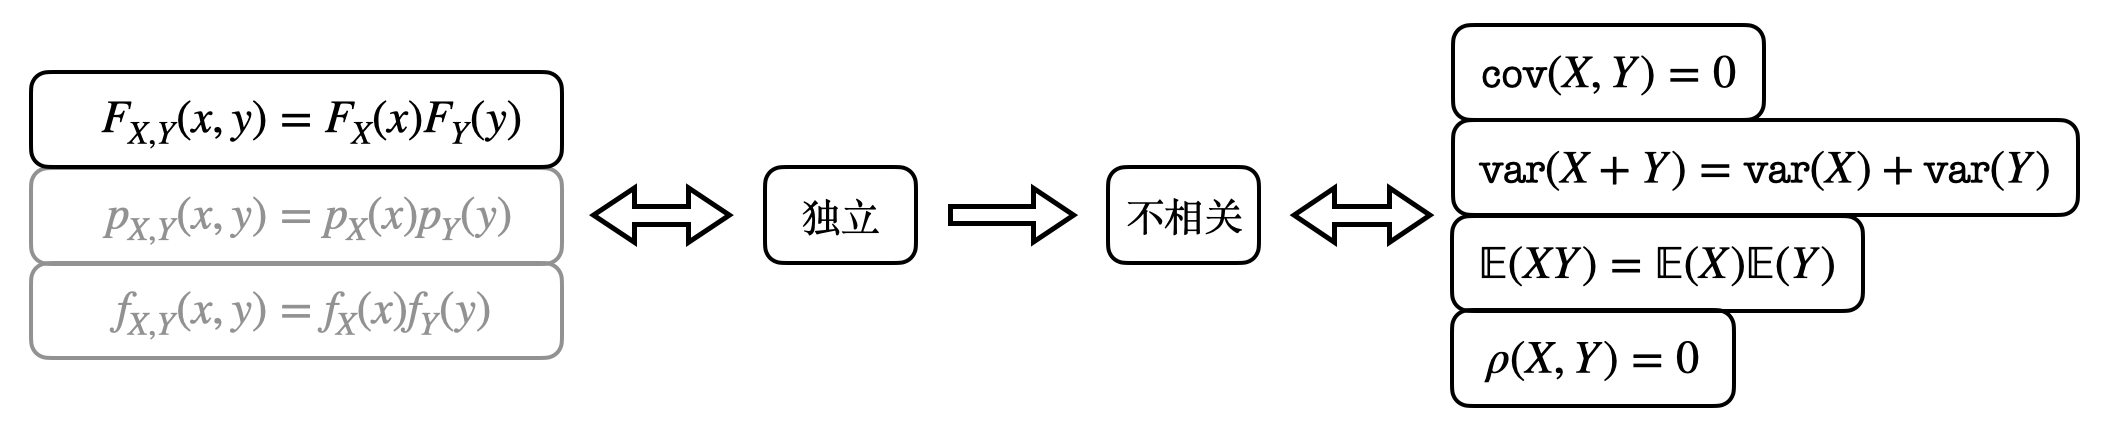
\includegraphics[width=0.9\linewidth]{figs/随机变量的独立性与相关性.png}
    \caption{随机变量的独立性与相关性示意图}
    \label{fig:independence-correlation}
\end{figure}

\begin{definition}[协方差与相关系数]
设 $X,Y$ 是两个随机变量,定义协方差与相关系数分别为:
\[
\cov(X,Y)=\E [(X-\E  X)(Y-\E  Y)],\quad\rho(X,Y)=\frac{\cov(X,Y)}{\sqrt{\var X\var Y}}
\]
当 $\cov(X,Y)=\rho(X,Y)=0$ 时,称 $X$ 和 $Y$ 不相关。
\end{definition}

\begin{property}
从定义出发容易证明以下性质:
\begin{itemize}
    \item $\cov(X,X)=\var(X)$
    \item $\cov(X,aY+b)=a\cdot\cov(X,Y)$ 
    \item $\cov(X,Y+Z)=\cov(X,Y)+\cov(X,Z)$
\end{itemize}
\end{property}

\begin{property}
$|\rho(X,Y)|\leq 1$.
\end{property}
\begin{proof}
对 $\forall t\in \R$,由于 $\var(Y-tX)=t^2\var X-2t\cov(X,Y)+\var Y\geq 0$,所以:
\[\Delta=4\cov^2(X,Y)-4\var X\var Y\leq 0\]
即有 $|\rho(X,Y)|\leq 1$.
\end{proof}

\begin{theorem}
设 $X,Y$ 是两个随机变量,则:
\[\cov(X,Y)=\E[XY]-\E X\E Y\]
\end{theorem}
\begin{proof}
\begin{align*}
\cov(X,Y)&=\E[(X-\E X)(Y-\E Y)]\\
&=\E[XY-\E X\cdot Y-X\cdot \E Y+\E X\E Y]\\
&=\E[XY]-\E X\cdot\E Y-\E X\cdot\E Y+\E X\cdot\E Y\\
&=\E[XY]-\E X\E Y
\end{align*}
\end{proof}

\begin{corollary}[独立与相关]
设 $X,Y$ 是两个随机变量,若 $X,Y$ 独立,则 $X,Y$ 不相关。
\end{corollary}
\begin{note}
反之不成立,不相关不能推出独立。
\end{note}

\begin{example}[不相关且不独立]
设随机变量 $X,Y$ 以 $1/4$ 的概率取 $(1,0),(0,1),(-1,0),(0,-1)$,则 $\E X=\E Y=\E[XY]=0$,于是 $\cov(X,Y)=\E[XY]-\E X\E Y=0$,故 $X,Y$ 不相关。但是 $p_{X,Y}(1,0)=1/4\neq p_X(1)p_Y(0)=1/4\cdot 1/2=1/8$,故二者不独立。直观上,$X$ 取非零值就要求 $Y$ 取零值,因此不独立。
\end{example}

\begin{theorem}[随机变量和的方差]
设随机变量 $X,Y$ 有有限的方差,则:
\[\var(X+Y)=\var X+2\cov(X,Y)+\var Y\]
更一般的,设随机变量 $X_1,X_2,\ldots,X_n$ 有有限的方差,则:
\[
\var\left(\sum_{i=1}^n X_i\right)=\sum_{i=1}^n\var(X_i)+\sum_{\{(i,j)\mid i\neq j\}}\cov(X_i,X_j)
\]
\end{theorem}
\begin{proof}
设 $\tilde X_i=X_i-\E[X_i]$,则:
\begin{align*}
\var\left(\sum_{i=1}^n X_i\right)&=\E\left[\left(\sum_{i=1}^n{\tilde X_i}^2\right)^2\right]\\
&=\E\left[\sum_{i=1}^n\sum_{j=1}^n\tilde X_i\tilde X_j\right]\\
&=\sum_{i=1}^n\sum_{j=1}^n\E\left[\tilde X_i\tilde X_j\right]\\
&=\sum_{i=1}^n\E[{\tilde X_i}^2]+\sum_{\{(i,j)\mid i\neq j\}}^n\E\left[\tilde X_i\tilde X_j\right]\\
&=\sum_{i=1}^n\var(X_i)+\sum_{\{(i,j)\mid i\neq j\}}\cov(X_i,X_j)
\end{align*}
\end{proof}

\begin{corollary}
设随机变量 $X,Y$ 有有限的方差,$a,b$ 为常数,则:
\[
\var(aX+bY)=a^2\var X+2ab\cov(X,Y)+b^2\var Y
\]
或写作矩阵形式:
\[
\var(aX+bY)=\begin{bmatrix}a&b\end{bmatrix}\begin{bmatrix}\var X&\cov(X,Y)\\\cov(Y,X)&\var Y\end{bmatrix}\begin{bmatrix}a\\b\end{bmatrix}
\]
\end{corollary}

% \begin{property}
% $\var(X)=0\implies \mathbb P(X=\E  X)=1$
% \end{property}
% \begin{proof}
% 根据切比雪夫不等式(见后文),$\mathbb P\left(|X-\E  X|\geq \frac{1}{n}\right)\leq n^2\var(X)=0$ 对 $\forall n$ 都成立,故 $\mathbb P(X=\E  X)=1$.
% \end{proof}

\subsection{再论条件期望与条件方差}
\label{sec:cond-e-cond-var}

\begin{definition}[条件期望作为估计量]
设 $X,Y$ 是随机变量,若将 $Y$ 视作能提供关于 $X$ 的信息的观测值,则可将条件期望视为给定 $Y$ 下对 $X$ 的估计,记作:
\[
\hat X=\E[X\vert Y]
\]
注意 $\hat X$ 是随机变量 $Y$ 的函数。进一步地,记估计误差为:
\[
\tilde X=\hat X-X
\]
则 $\tilde X$ 是随机变量 $X,Y$ 的二元函数。
\end{definition}

\begin{property}
根据全期望公式易知,条件期望是无偏估计,即 $\E\hat X=\E X$,或 $\E\tilde X=0$.
\end{property}

\begin{property}
$\E[\tilde X\vert Y]=0$,即对任意 $y$,都有 $\E[\tilde X\vert Y=y]=0$.
\end{property}
\begin{proof}
\[
\E[\tilde X\vert Y]=\E[(\hat X-X)\vert Y]=\E[\hat X\vert Y]-\E[X\vert Y]=\hat X-\hat X=0
\]
\end{proof}

\begin{property}
估计量 $\hat X$ 与估计误差 $\tilde X$ 不相关。
\end{property}
\begin{proof}
\[
\E[\hat X\tilde X]=\E[\E[\hat X\tilde X\vert Y]]=\E[\hat X\E[\tilde X\vert Y]]=0=\E\hat X\E\tilde X
\]
\end{proof}

\begin{property}
$\var(X)=\var(\hat X)+\var(\tilde X)$.
\end{property}
\begin{proof}
由于 $\hat X$ 与 $\tilde X$ 不相关,故 $\cov(\hat X,\tilde X)=0$,又 $X=\hat X+\tilde X$,故:
\[
\var(X)=\var(\hat X)+2\cov(\hat X,\tilde X)+\var(\tilde X)=\var(\hat X)+\var(\tilde X)
\]
\end{proof}


\subsection{矩母函数}

\begin{definition}[矩母函数]
设 $X$ 是一个随机变量,定义其矩母函数为:
\[
M_X(s)=\E[e^{sX}]=\begin{dcases}
    \sum_x e^{sx}p_X(x),&\text{$X$ 离散}\\
    \int_{-\infty}^{\infty} e^{sx}f_X(x)\mathrm dx,&\text{$X$ 连续}
\end{dcases}
\]
其定义域为使得 $\E[e^{sX}]$ 存在的 $s$. 在上下文清晰时可简记作 $M(s)$.
\end{definition}

\begin{theorem}[矩母函数计算矩]
设随机变量 $X$ 的矩母函数为 $M(s)$,则:
\[
\left.\frac{\mathrm d^n}{\mathrm ds^n}M(s)\right|_{s=0}=\E[X^n]
\]
\end{theorem}
\begin{proof}
假设积分(期望)与微分可交换,则:
\[
\frac{\mathrm d^n}{\mathrm ds^n}M(s)=\frac{\mathrm d^n}{\mathrm ds^n}\E[e^{sX}]=\E\left[\frac{\mathrm d^n}{\mathrm ds^n}e^{sX}\right]=\E[X^ne^{sX}]
\]
代入 $s=0$ 得:
\[
\left.\frac{\mathrm d^n}{\mathrm ds^n}M(s)\right|_{s=0}=\E[X^n]
\]
\end{proof}

\begin{theorem}[矩母函数与分布]
若随机变量 $X$ 的矩母函数 $M_X(s)$ 满足:存在一个正数 $a$,使得对 $\forall s\in[-a,a]$,$M_X(s)$ 都是有限的,则矩母函数 $M_X(s)$ 唯一决定 $X$ 的分布函数。
\end{theorem}

\begin{theorem}[独立随机变量之和]
设 $X,Y$ 是独立随机变量,$Z=X+Y$,则:
\[M_Z(s)=M_X(s)M_Y(s)\]
\end{theorem}
\begin{proof}
\[
M_Z(s)=\E[e^{sZ}]=\E[e^{s(X+Y)}]=\E[e^{sX}e^{sY}]=\E[e^{sX}]\E[e^{sY}]=M_X(s)M_Y(s)
\]
\end{proof}
\begin{corollary}
设 $X_1,X_2,\ldots,X_n$ 是独立随机变量,$Z=X_1+X_2+\cdots+X_n$,则:
\[
M_Z(s)=M_{X_1}(s)M_{X_2}(s)\cdots M_{X_n}(s)
\]
\end{corollary}

\begin{definition}[多元矩母函数]
设 $X_1,X_2,\ldots,X_n$ 是随机变量,定义它们的多元矩母函数为:
\[
M_{X_1,X_2,\ldots,X_n}(s_1,s_2,\ldots,s_n)=\E[e^{s_1X_1+s_2X_2+\cdots+s_nX_n}]
\]
\end{definition}


\subsection{随机个随机变量之和}

\begin{theorem}[随机个随机变量之和的期望、方差与矩母函数]
设 $N$ 是取正整数值的随机变量,$X_1,X_2,\ldots$ 是独立同分布的随机变量,且 $N,X_1,X_2,\ldots$ 相互独立(即这些随机变量的任意有限子集都是独立的)。设 $Y=X_1+X_2+\cdots+X_N$,则:
\begin{gather*}
    \E Y=\E N\E X\\
    \var(Y)=\E N\var(X)+(\E X)^2\var(N)\\
    M_Y(s)=\sum_{n=1}^\infty (M_X(s))^n p_N(n)
\end{gather*}
其中 $\E X,\var(X),M_X(s)$ 表示各 $X_i$ 的期望、方差和矩母函数。
\end{theorem}
\begin{proof}
给定正整数 $n$,随机变量 $X_1+X_2+\cdots+X_n$ 与 $N$ 独立,故与事件 $\{N=n\}$ 独立,故:
\begin{align*}
\E[Y\vert N=n]&=\E[X_1+X_2+\cdots+X_N\vert N=n]\\
&=\E[X_1+X_2+\cdots+X_n\vert N=n]\\
&=\E[X_1+X_2+\cdots+X_n]\\
&=n\E X
\end{align*}
这对于任意非负整数 $n$ 都成立,因此:
\[
\E[Y\vert N]=N\E X
\]
于是根据全期望公式,有:
\[
\E Y=\E[\E[Y\vert N]]=\E[N\E X]=\E N\E X
\]
类似地,给定正整数 $n$,有:
\begin{align*}
\var(Y\vert N=n)&=\var(X_1+X_2+\cdots+X_N\vert N=n)\\
&=\var(X_1+X_2+\cdots+X_n\vert N=n)\\
&=\var(X_1+X_2+\cdots+X_n)\\
&=n\var(X)
\end{align*}
这对任意正整数 $n$ 都成立,因此:
\[
\var(Y\vert N)=N\var(X)
\]
于是根据全方差公式,有:
\begin{align*}
\var(Y)&=\E[\var(Y\vert N)]+\var(\E[Y\vert N])\\
&=\E[N\var(X)]+\var(N\E X)\\
&=\E N\var(X)+(\E X)^2\var(N)
\end{align*}
类似地,给定正整数 $n$,有:
\begin{align*}
\E[e^{sY}\vert N=n]&=\E[e^{s(X_1+X_2+\cdots+X_N}\vert N=n]\\
&=\E[e^{s(X_1+X_2+\cdots+X_n}\vert N=n]\\
&=\E[e^{s(X_1+X_2+\cdots+X_n}]\\
&=\E[e^{sX_1}]\E[e^{sX_2}]\cdots\E[e^{sX_n}\\
&=(M_{X}(s))^n
\end{align*}
上式对任意正整数 $n$ 都成立,因此:
\[
\E[e^{sY}\vert N]=(M_X(s))^N
\]
于是根据全期望公式,有:
\[
M_Y(s)=\E[e^{sY}]=\E[\E[e^{sY}\vert N]]=\E[(M_X(s))^N]=\sum_{n=1}^\infty (M_X(s))^n p_N(n)
\]
\end{proof}

\begin{com}
对比 $M_Y(s)$ 与 $M_N(s)$:
\begin{gather*}
    M_Y(s)=\sum_{n=1}^\infty (M_X(s))^n p_N(n)\\
    M_N(s)=\sum_{n=1}^\infty (e^s)^np_N(n)
\end{gather*}
可以看见 $M_Y(s)$ 就是将 $M_N(s)$ 中的函数 $e^s$ 替换为 $X_i$ 的矩母函数 $M_X(s)$.
\end{com}
 \pagebreak
\section{极限理论}

给定一列独立同分布随机变量 $X_1,X_2,\ldots$,定义前 $n$ 项和 $S_n=X_1+X_2+\cdots+X_n$,本章的极限理论研究 $S_n$ 及其相关变量在 $n\to\infty$ 时的极限性质。


\subsection{马尔可夫不等式与切比雪夫不等式}

\begin{theorem}[马尔可夫不等式]
设随机变量 $X$ \textbf{只取非负值},则对任意 $a>0$,有:
\[
\mathbb P(X\geq a)\leq \frac{\mathbb EX}{a}
\]
\end{theorem}
\begin{com}
粗略来讲,马尔可夫不等式指出,一个非负随机变量如果均值很小,那么该随机变量取大值的概率也很小。
\end{com}
\begin{proof}
这里假设 $X$ 是连续随机变量,离散类似。
\[
\mathbb EX=\int_0^{+\infty}xf_X(x)\mathrm dx\geq \int_a^{+\infty}xf_X(x)\mathrm dx\geq a\int_a^{+\infty}f_X(x)\mathrm dx=a\cdot\mathbb P(X\geq a)
\]
\end{proof}

\begin{example}
\label{ex:markov}
设 $X\sim U(0,4)$,则 $\E X=2$,由马尔可夫不等式可得:
\[
\Pb(X\geq2)\leq\frac{2}{2}=1,\quad\Pb(X\geq 3)\leq\frac{2}{3},\quad\Pb(X\geq 4)\leq\frac{2}{4}=\frac{1}{2}
\]
而真实概率是:
\[
\Pb(X\geq2)=\frac{1}{2},\quad\Pb(X\geq 3)=\frac{1}{4},\quad\Pb(X\geq 4)=0
\]
可见由马尔可夫不等式给出的上界非常的粗糙。
\end{example}

\begin{theorem}[切比雪夫不等式]
设随机变量 $X$ 的均值为 $\mu$,方差为 $\sigma^2$,则对任意 $c>0$,有:
\[
\mathbb P(|X-\mu|\geq c)\leq \frac{\sigma^2}{c^2}
\]
\end{theorem}
\begin{com}
粗略来讲,切比雪夫不等式指出,如果一个随机变量的方差非常小,那么该随机变量取远离均值的概率也非常小。
\end{com}
\begin{proof}
利用马尔可夫不等式,
\[
\mathbb P(|X-\mu|\geq c)=\mathbb P((X-\mu)^2\geq c^2)\leq \frac{\mathbb E[(X-\mu)^2]}{c^2}=\frac{\sigma^2}{c^2}
\]
\end{proof}

相比马尔可夫不等式,切比雪夫不等式利用了随机变量的方差的信息,因此会更准确。不过均值和方差也仅仅是粗略描述了随机变量的性质,因此它给出的上界可能依旧距离精确概率较远。

\begin{example}
仍然考虑例 \ref{ex:markov},即 $X\sim U(0,4),\,\E X=2,\,\var X=\frac{4}{3}$,则根据切比雪夫不等式有:
\[
\Pb(|X-2|\geq1)\leq\frac{4}{3}
\]
由于概率一定小于等于 1,所以这个不等式并没有带来任何信息。
\end{example}

\begin{example}
设 $X\sim E(1)$,则 $\E X=\var X=1$,对任意 $c>2$,应用切比雪夫不等式可得:
\[
\Pb(X\geq c)=\Pb(X-1\geq c-1)=\Pb(|X-1|\geq c-1)\leq\frac{1}{(c-1)^2}
\]
而真实概率是 $\Pb(X\geq c)=e^{-c}$,可见切比雪夫不等式给出的上界比较保守。
\end{example}


\subsection{弱大数定律}

\begin{definition}[依概率收敛]
设 $X_1,X_2,\ldots$ 是随机变量序列,$a\in\mathbb R$,若对任意 $\epsilon>0$,都有:
\[
\lim_{n\to\infty}\Pb(|X_n-a|\geq\epsilon)=0
\]
则称 $\{X_n\}$ 依概率收敛到 $a$.
\end{definition}

\begin{com}
用 $\epsilon$-$N$ 语言描述上述定义中的数列极限,则依概率收敛可以等价叙述为:对任意 $\epsilon>0$ 和 $\delta>0$,存在 $N\in\mathbb N$,当 $n\geq N$ 时,都有:
\[
\Pb(|X_n-a|\geq\epsilon)\leq\delta
\]
其中 $\epsilon$ 称作精度,$\delta$ 称作置信水平。
\end{com}

\begin{theorem}[弱大数定律]
设 $X_1,X_2,\ldots$ 是独立同分布的随机变量序列,其公共分布均值为 $\mu$,则样本均值 $M_n=\frac{1}{n}\sum_{i=1}^nX_i$ 依概率收敛到 $\mu$,即对任意 $\epsilon>0$,有:
\[
\lim_{n\to\infty}\mathbb P(|M_n-\mu|\geq\epsilon)=0
\]
\end{theorem}
\begin{proof}
这里仅对方差有界的情形进行证明,方差无界时弱大数定律依然成立,但是证明较为精巧。
考虑 $M_n$ 的均值和方差:
\begin{align*}
&\mathbb EM_n=\frac{1}{n}\sum_{i=1}^n\mathbb EX_i=\mu\\
&\text{var}(M_n)=\frac{1}{n^2}\sum_{i=1}^n\text{var}(X_i)=\frac{\sigma^2}{n}
\end{align*}
于是根据切比雪夫不等式,对任意 $\epsilon>0$,有:
\[
\mathbb P(|M_n-\mu|\geq\epsilon)\leq \frac{\sigma^2}{n\epsilon^2}\to0\quad(n\to\infty)
\]
\end{proof}
\begin{com}
一般情形的弱大数定理称为辛钦大数定律,而方差有界的情形称之为切比雪夫大数定律。
更特殊的,对于 $X_1,X_2,\ldots\overset{\text{i.i.d.}}{\sim}B(1,p)$ 的情形而言,我们称之为伯努利大数定律:
\[
\lim_{n\to\infty}\mathbb P(|M_n-p|\geq \epsilon)=0
\]
\end{com}


\subsection{中心极限定理}

\begin{theorem}[中心极限定理]
设 $X_1,X_2,\ldots$ 是独立同分布的随机变量序列,序列的每一项的均值为 $\mu$,方差为 $\sigma^2$,则对 $\forall x\in\R$,有:
\[
\lim_{n\to\infty}\mathbb P\left(\frac{\sum\limits_{i=1}^nX_i-n\mu}{\sqrt n\sigma}\leq  x\right)=\Phi(x)
\]
其中 $\Phi(x)$ 表示标准正态分布的 CDF.
\end{theorem}
\begin{com}
粗略来讲,中心极限定理表明,在大样本的情况下,独立同分布的随机变量序列的样本均值的标准化结果服从标准正态分布。
\end{com}

\begin{com}
这个一般情形的定理被称作林德伯格-莱维中心极限定理。
\end{com}

\begin{com}
对于 $X_1,X_2,\ldots\overset{\text{i.i.d.}}{\sim} B(1,p)$ 的特殊情形而言,我们称之为棣莫弗-拉普拉斯中心极限定理:
\[
\lim_{n\to\infty}\mathbb P\left(\frac{\sum\limits_{i=1}^nX_i-np}{\sqrt{np(1-p)}}\leq x\right)=\Phi(x)
\]
\end{com}


\subsection{强大数定律}

\begin{definition}[以概率 1 收敛/几乎必然收敛]
设 $X_1,X_2,\ldots$ 是随机变量序列,$a\in\mathbb R$,若:
\[
\Pb\left(\lim_{n\to\infty}X_n=a\right)=1
\]
则称 $\{X_n\}$ 以概率 1 收敛到 $a$ 或几乎必然收敛到 $a$.
\end{definition}

\begin{theorem}[强大数定律]
设 $X_1,X_2,\ldots$ 是均值为 $\mu$ 的独立同分布的随机变量序列,则样本均值 $M_n=\frac{1}{n}\sum_{i=1}^nX_i$ 以概率 1 收敛到 $\mu$,即:
\[
\Pb\left(\lim_{n\to\infty}M_n=\mu\right)=1
\]
\end{theorem}

\begin{com}
弱大数定律是指 $M_n$ 显著性偏离 $\mu$ 的事件的概率在 $n\to\infty$ 时趋于 0,但是对任意有限的 $n$,这个概率可以是正的。所以可以想象的是,在 $M_n$ 这个无穷的序列中,常常有 $M_n$ 显著偏离 $\mu$. 而强大数定律则进一步告诉我们,这样的显著偏离事件只能发生有限次。
\end{com}
 \pagebreak
\section{特征值的估计}

\subsection{特征值的估计}

矩阵的特征值在理论上和实际应用中都是十分重要的,但是特征值的计算一般是非常麻烦的,尤其当矩阵的阶数比较高时,要精确计算出矩阵的特征值是相当困难的,因此,由矩阵元素的简单关系式估计出特征值的范围就显得尤为重要。本节将主要给出特征值的估计与圆盘定理,以及谱半径的估计。

\begin{theorem}[特征值的上界]
设 $A\in \mathbb R^{n\times n}$,令:
\[
    M=\max_{1\leq r,s\leq n}\frac{1}{2}|a_{rs}-a_{sr}|
\]
若 $\lambda$ 表示 $A$ 的任一特征值,则 $\lambda$ 的虚部 $\text{Im}(\lambda)$ 满足不等式:
\begin{align*}
    &|\text{Im}(\lambda)|\leq M\sqrt{\frac{n(n-1)}{2}}\\
    &|\text{Im}(\lambda)|\leq\frac{\Vert A-A^T\Vert_2}{2}\\
    &|\text{Im}(\lambda)|\leq\frac{\Vert A-A^T\Vert_1\cdot\sqrt{n}}{2}
\end{align*}
\end{theorem}

\begin{remark}
基本思想:任何一个实方阵都可以拆分为实对称阵和实反对称阵的和:
\[
    A=\frac{1}{2}(A+A^T)+\frac{1}{2}(A-A^T)
\]
我们知道实对称阵的特征值一定是实数,而实反对称阵的特征值一定是 0 或虚数。因此,可以认为上面的两部分分别决定了特征值的实部和虚部,这就是为什么我们关注 $M=\max\limits_{1\leq r,s\leq n}\frac{1}{2}|a_{rs}-a_{sr}|$.
\end{remark}
\begin{proof}
暂略。
\end{proof}

\begin{definition}[行对角占优]
设 $A\in\mathbb C^{n\times n}$,令:
\[
    R_r(A)=\sum_{s=1,s\neq r}^n|a_{rs}|,\quad r=1,\ldots,n
\]
若 $|a_{rr}|>R_{r}(A),\ \forall\ r=1,\ldots,n$,则称矩阵 $A$ 按行对角占优。
\end{definition}

\begin{theorem}
行对角占优阵一定可逆。
\end{theorem}
\begin{proof}
假设 $A$ 不可逆,则其列线性相关,即存在不全为零的 $k_1,\ldots,k_n$ 使得 $k_1a_1+\cdots+k_na_n=0$. 设 $k_r$ 是其中模长最大的,考虑第 $r$ 个分量:
\[
    k_1a_{r1}+\cdots+k_na_{rn}=0\implies a_{rr}=-\sum_{s=1,s\neq r}^n\frac{k_s}{k_r}a_{rs}
\]
于是:
\[
    |a_{rr}|\leq \sum_{s=1,s\neq r}^n\frac{|k_s|}{|k_r|}|a_{rs}|\leq \sum_{s=1,s\neq r}^n|a_{rs}|
\]
与 $A$ 行对角占优矛盾,故假设不成立。
\end{proof}

\begin{theorem}[行对角占优阵的行列式的上下界]
设 $A\in\mathbb C^{n\times n}$ 且按行对角占优,令:
\[
    M_r=|a_{rr}|+\sum_{s=r+1}^n|a_{rs}|,\quad m_r=|a_{rr}|-\sum_{s=r+1}^n|a_{rs}|,\quad r=1,\ldots,n
\]
则:
\[
    0<\prod_{r=1}^n m_r\leq |\det A|=\prod_{r=1}^n|\lambda_r(A)|\leq\prod_{r=1}^n M_r
\]
当 $a_{rs}=0\ (s>r)$ 时等号成立。
\end{theorem}
\begin{proof}
对 $A$ 分块:
\[
    A=\left[\begin{array}{c:ccc}
    a_{11}&a_{12}&\cdots&a_{1n}\\
    \hdashline a_{21}&&&\\
    \vdots&&A_1&\\
    a_{n1}&&&\\
    \end{array}\right]
\]
设 $x=(\xi_2,\ldots,\xi_n)^T$ 且满足:
\[
    \begin{bmatrix}a_{21}\\\vdots\\a_{n1}\end{bmatrix}+A_1\begin{bmatrix}\xi_2\\\vdots\\\xi_n\end{bmatrix}=0
\]
则有 $|\xi_k|=\max\{|\xi_2|,\ldots,|\xi_n|\}<1$,证明方式与上面证明行对角占优矩阵一定可逆的方式类似。
于是,利用行列式的性质,有:
\[
    \det(A)=\det\left(A\begin{bmatrix}1&0\\x&I_{n-1}\end{bmatrix}\right)=\det\left(
    \left[\begin{array}{c:ccc}
    b_{11}&a_{12}&\cdots&a_{1n}\\
    \hdashline&&&\\
    0&&A_1&\\
    &&&
    \end{array}\right]
    \right)=|b_{11}|\cdot\det(A_1)
\]
其中
\[
    b_{11}=a_{11}+\sum_{s=2}^na_{1s}\xi_s,\quad|\xi_s|<1
\]
因此 $m_1\leq|b_{11}|\leq M_1$.  然后递归地对 $A_1$ 做类似推导即可。
\end{proof}

\begin{theorem}[Hadamard 不等式]
设 $A\in\mathbb C^{n\times n}$,则有:
\[
    |\det(A)|=\prod_{r=1}^n|\lambda_r(A)|\leq\left[\prod_{s=1}^n\left(\sum_{r=1}^n|a_{rs}|^2\right)\right]^{1/2}
\]
\end{theorem}
\begin{remark}[直观解释]
平行多面体的体积小于等于将其拉成正立方体的体积。
\end{remark}
\begin{proof}
若 $a_1,\ldots,a_n$ 线性无关,则显然成立;否则,进行 Gram-Schmidt 正交化过程,写作矩阵形式:
\[
    (a_1,a_2,\ldots,a_n)=(b_1,b_2,\ldots,b_n)\begin{bmatrix}1&k_{21}&\cdots&k_{n1}\\&1&\cdots&k_{n2}\\&&\ddots&\vdots\\&&&1\end{bmatrix}
\]
易知 $\Vert a_i\Vert^2\geq\Vert b_i\Vert^2$,于是:
\[
    |\det(A)|^2=|\det(B)|^2=\det(B^HB)=\Vert b_1\Vert^2\cdots\Vert b_n\Vert^2\leq\Vert a_1\Vert^2\cdots\Vert a_n\Vert^2
\]
\end{proof}

\begin{theorem}[Schur 不等式,特征值模长平方和的界]
设 $A\in\mathbb C^{n\times n}$ 的特征值为 $\lambda_1,\ldots,\lambda_n$,则:
\[
    \sum_{r=1}^n|\lambda_r|^2\leq\sum_{r=1}^n\sum_{s=1}^n|a_{rs}|^2=\Vert A\Vert_F^2
\]
\end{theorem}
\begin{proof}
根据 Schur 定理 \ref{thm:schur},存在酉矩阵 $U$ 使得 $A=UTU^H$,其中 $T$ 为上三角矩阵,对角元素为 $A$ 的特征值,且:
\[
    \sum_{r=1}^n|\lambda_r|^2=\sum_{k=1}^n|t_{kk}|^2\leq\sum_{r=1}^n\sum_{s=1}^n|t_{rs}|^2=\text{tr}(T^HT)=\text{tr}(A^HA)
\]
\end{proof}

\begin{definition}[行盖尔圆]
设 $A\in\mathbb C^{m\times n}$,记第 $i$ 个行盖尔圆为:
\[
    S_i=\{z\mid |z-a_{ii}|\leq R_i,\,z\in\mathbb C\}
\]
其中 $R_i=R_i(A)=\sum_{j\neq i}|a_{ij}|$.
\end{definition}

\begin{theorem}[圆盘定理 1]
$A$ 的所有特征值在其 $n$ 个盖尔圆的并集之内,即:
\[
    \lambda\in S=\bigcup_{i=1}^nS_i=\bigcup_{i=1}^n\{z\mid |z-a_{ii}|\leq R_i,\,z\in\mathbb C\}
\]
\end{theorem}
\begin{proof}
设 $Ax=\lambda x$,写作分量形式:
\[
    \sum_{j=1}^na_{ij}x_j=\lambda x_i\implies (\lambda-a_{ii})x_i=\sum_{j\neq i}a_{ij}x_j
\]
设 $x_t$ 为 $x$ 各分量中模最大的那个,则 $x_t\neq 0$,上式取 $i=t$ 后两边同时除以 $x_t$ 并取模得:
\[
    |\lambda-a_{tt}|=\sum_{j\neq t}|a_{tj}|\left|\frac{x_j}{x_t}\right|\leq\sum_{j\neq t}|a_{tj}|=R_t(A)
\]
因此 $\lambda\in S_t$.  于是任意特征值 $\lambda\in\bigcup_{i=1}^n S_i$.
\end{proof}

\begin{remark}
圆盘定理 1 说明,特征值 $\lambda$ 属于特征向量最大分量的下标对应的盖尔圆。
\end{remark}

\begin{theorem}[圆盘定理 2]
设矩阵 $A$ 的 $n$ 个盖尔圆有 $k$ 个互相连通并且与其余 $n-k$ 个不相交,则这个连通区域中恰有 $k$ 个特征值。
\end{theorem}
\begin{remark}
设 $A=D+B$,其中 $D$ 为对角矩阵。设 $A(t)=D+tB$,则当 $t=0$ 时,所有盖尔圆都是点,也就是特征值;当 $t$ 从 $0$ 到 $1$ 连续变化时,盖尔圆越来越大,而特征值也是\textbf{连续}变化的,所以 $t=1$ 时特征值只能在其连通区域内,不可能跳跃到不连通的另一个区域中。从这个角度也可以知道,当两个盖尔圆相切时,其特征值最多到达切点处。
\end{remark}

\begin{corollary}
若 $n$ 阶矩阵 $A$ 的 $n$ 个盖尔圆两两互不相交(都是孤立的),则 $A$ 相似于对角矩阵。
\end{corollary}

\begin{corollary}
设 $n$ 阶实矩阵 $A$ 的 $n$ 个盖尔圆两两互不相交,则 $A$ 的特征值全为实数。
\end{corollary}

\begin{proof}
由于 $A$ 为实矩阵,故所有盖尔圆的圆心都在实轴上。若 $A$ 有复特征值,则必有与之关于实轴对称的共轭复对称值,与其在同一个盖尔圆中。由于盖尔圆两两互不相交,且一个孤立盖尔圆内只能有一个特征值,所以 $A$ 的特征值只能都是实数。
\end{proof}

\begin{definition}[列盖尔圆]
设 $A\in\mathbb C^{m\times n}$,记第 $j$ 个列盖尔圆为:
\[
    G_j=\{z\mid |z-a_{jj}|\leq R'_j,\,z\in\mathbb C\}
\]
其中 $R'_j=R'_j(A)=\sum_{i\neq j}|a_{ij}|$.
\end{definition}

\begin{corollary}
列盖尔圆有与行盖尔圆类似的圆盘定理。结合二者可知,$A$ 的所有特征值都在以下平面区域之中:
\[
T=\left(\bigcup_{i=1}^nS_i\right)\cap\left(\bigcup_{j=1}^nG_j\right)
\]
\end{corollary}

\begin{theorem}
相似矩阵的盖尔圆的圆心相同、半径不同。
\end{theorem}
\begin{proof}
由于 $B=P^{-1}AP$ 的第 $i$ 行第 $j$ 列元素为 $a_{ij}p_i/p_j$,所以对于 $B$:
\[
    R_i=\sum_{j\neq i}\left\vert a_{ij}\cdot\frac{p_i}{p_j}\right\vert
\]
而圆心依旧是 $a_{ii}\cdot p_i/p_i=a_{ii}$.
\end{proof}

\begin{remark}
这个定理可以用于隔离特征值:取 $P=\text{diag}(p_1,\ldots,p_n),\,p_i>0$,若想要缩小半径,则将对应元素设置得大一些,这样原本相交的盖尔圆就能被隔离开了。
\end{remark}

\begin{theorem}
设 $A$ 为 $n$ 阶正规矩阵,则:
\[
    \rho(A)=\Vert A\Vert_2=\sqrt{\lambda_{A^HA}}
\]
其中 $\lambda_{A^HA}$ 为 $A^HA$ 的最大特征值。
\end{theorem}
\begin{proof}
设 $A$ 的特征值为 $\lambda_1,\ldots,\lambda_n$,存在酉矩阵 $U$ 使得:
\[
    U^HAU=\text{diag}(\lambda_1,\ldots,\lambda_n)
\]
于是:
\[
    U^HA^HU=\text{diag}(\bar\lambda_1,\ldots,\bar\lambda_n)
\]
因此:
\[
    U^HA^HAU=\text{diag}(|\lambda_1|^2,\ldots,|\lambda_n|^2)
\]
故 $A^HA$ 的特征值为 $|\lambda_1|^2,\ldots,|\lambda_n|^2$,记 $\lambda_{A^HA}=\max_{1\leq i\leq n}|\lambda_i|^2$,则:
\[
    \Vert A\Vert_2=\sqrt{\lambda_{A^HA}}=\max_{1\leq i\leq n}|\lambda_i|=\rho(A)
\]
\end{proof}

\begin{remark}
由于实对称矩阵、实反对称矩阵、正交矩阵、酉矩阵、Hermite 矩阵、反 Hermite 矩阵、对角矩阵都是正规矩阵,所以它们都有性质 $\rho(A)=\Vert A\Vert_2$.
\end{remark}
\begin{remark}
事实上,从上述证明过程可以看出,正规矩阵的奇异值等于特征值的模长的平方(可以一一对应上)。
\end{remark}


\subsection{广义特征值问题}

\begin{definition}[广义特征值]
设 $A,B$ 为 $n$ 阶方阵,若存在数 $\lambda$,使得方程 $Ax=\lambda Bx$ 存在非零解,则称 $\lambda$ 为 $A$ 相对于 $B$ 的广义特征值,$x$ 为 $A$ 相对于 $B$ 的属于广义特征值 $\lambda$ 的特征向量。
\end{definition}

\noindent\textbf{广义特征值求解}:解 $(\lambda B-A)x=0\iff\det(\lambda B-A)=0$ 即可。注意这里的特征多项式 $\det(\lambda B-A)$ 不一定是 $n$ 阶多项式,从而不一定有 $n$ 个根。

\vskip 6pt \noindent\textbf{以下仅考虑 $A,B$ 是正定 Hermite 矩阵的情形}。

\begin{definition}[按 $B$ 标准正交化]
若向量系 $(x_1,\ldots,x_n)$ 满足:
\[
    (x_i,Bx_j)=\delta_{ij}
\]
称该向量系为按 $B$ 标准正交化的向量系。
\end{definition}

\begin{definition}[广义特征值的等价表述 1]
由于 $B$ 正定,因此可逆,故:
\[
    Ax=\lambda Bx\implies B^{-1}Ax=\lambda x
\]
转化为了标准特征值问题。但一般而言 $B^{-1}A$ 不再是 Hermite 矩阵。
\end{definition}

\begin{definition}[广义特征值的等价表述 2]
由于 $B$ 为 Hermite 矩阵,因此存在 Cholesky 分解,$B=GG^H$,其中 $G$ 满秩,于是:
\[
    Ax=\lambda Bx\implies Ax=\lambda GG^Hx
\]
令 $y=G^Hx$,则:
\[
    G^{-1}A(G^H)^{-1}y=\lambda y
\]
转化为了标准特征值问题,且 $G^{-1}A(G^H)^{-1}$ 仍然是 Hermite 矩阵,因此广义特征值为实数,设为 $\lambda_1\leq\cdots\leq\lambda_n$,且存在一组正交归一化的特征向量 $(y_1,\ldots,y_n)$,即:
\begin{align*}
    &G^{-1}A(G^H)^{-1}y_i=\lambda y_i\\
    &y_i^Hy_j=\delta_{ij}
\end{align*}
将 $y$ 还原为 $x$,则:
\[
    y_i^Hy_j=(G^Hx_i)^H(G^Hx_j)=x_i^HGG^Hx_j=x_i^HBx_j=\delta_{ij}
\]
即 $(x_1,\ldots,x_n)$ 按 $B$ 标准正交。
\end{definition}


\subsection{对称矩阵特征值的极性}

我们首先讨论实对称矩阵特征值的极性与 Rayleigh 商。本节中记实对称矩阵 $A$ 的特征值按大小排列为 $\lambda_1\leq\lambda_2\leq\cdots\leq\lambda_n$,对应\textbf{标准正交}特征向量系为 $p_1,p_2,\ldots,p_n$.

\begin{remark}
将 Rayleigh 商定义在实对称矩阵上是为了保证特征值一定是实数,这样才可以比较。
\end{remark}

\begin{definition}[Rayleigh 商]
设 $A$ 是 $n$ 阶实对称矩阵,$x\in\mathbb R^n$,定义矩阵 $A$ 的 Rayleigh 商为:
\[
    R(x)=\frac{x^TAx}{x^Tx},\quad x\neq 0
\]
\end{definition}
\begin{theorem}
设 $A$ 为实对称矩阵,则:
\[
    \min_{x\neq 0}R(x)=\lambda_1,\quad\max_{x\neq 0}R(x)=\lambda_n
\]
\end{theorem}
\begin{proof}[证明 1]
任取 $x\neq 0$,依标准正交特征向量系分解 $x=c_1p_1+\cdots+c_np_n$,则:
\[
    x^Tx=c_1^2+\cdots+c_n^2,\quad x^TAx=c_1^2\lambda_1+\cdots+c_n^2\lambda_n
\]
故:
\[
    R(x)=k_1\lambda_1+\cdots+k_n\lambda_n,\quad\text{where}\; k_i=\frac{c_i^2}{c_1^2+\cdots+c_n^2}
\]
容易推出 $\lambda_1\leq R(x)\leq\lambda_n$,且 $R(p_1)=\lambda_1,\,R(p_n)=\lambda_n$.
\end{proof}
\begin{proof}[证明 2(梯度法)]
取对数 $\ln R(x)=\ln (x^TAx)-\ln(x^Tx)$,求导并令为零:
\[
    \frac{\mathrm d\ln R(x)}{\mathrm dx}=\frac{2Ax}{x^TAx}-\frac{2x}{x^Tx}=0\implies Ax=R(x)x
\]
因此极值点处 $R(x)$ 为 $A$ 的特征值,$x$ 为对应特征向量。于是最小值为最小特征值 $\lambda_1$,最大值为最大特征值 $\lambda_n$.
\end{proof}
\begin{proof}[证明 3(拉格朗日乘子法)]
原问题可等价转换为如下带约束优化问题:
\[
    \min_{x^Tx=1} x^TAx,\quad\max_{x^Tx=1} x^TAx
\]
引入拉格朗日函数:
\[
    L(x,\lambda)=x^TAx-\lambda x^Tx
\]
求导并令为零:
\[
    \frac{\partial L(x,\lambda)}{\partial x}=2Ax-2\lambda x=0\implies Ax=\lambda x
\]
这意味着极值点 $x$ 为 $A$ 的特征向量,$\lambda$ 是对应特征值。此时,极值正好也是 $x^TAx=\lambda x^Tx=\lambda$. 因此,原问题最小值就是 $A$ 的最小特征值 $\lambda_1$,最大值就是 $A$ 的最大特征值 $\lambda_n$.
\end{proof}

\begin{remark}
由于 $x$ 模长不影响 $R(x)$,所以上述定理也常常写作:
\[
    \min_{\Vert x\Vert_2=1}x^TAx=\lambda_1,\quad\max_{\Vert x\Vert_2=1}x^TAx=\lambda_n
\]
下文视情况两种写法都可能出现。
\end{remark}

\begin{theorem}[Rayleigh 商中的向量扩展为矩阵]
设 $A$ 为实对称矩阵,则对于任意的 $1\leq r\leq n$ 有:
\[
    \min_{X^TX=I_r}\text{tr}(X^TAX)=\lambda_1+\cdots+\lambda_r
\]
\end{theorem}
\begin{proof}
对 $A$ 作谱分解 $A=P\Lambda P^T$,其中 $P$ 为正交矩阵,$\Lambda=\text{diag}(\lambda_1,\ldots,\lambda_n)$. 记 $B=P^TX$,则问题转化为对角矩阵情形,即求证:
\[
    \min_{B^TB=I_r}\text{tr}(B^T\Lambda B)=\lambda_1+\cdots+\lambda_r
\]
记 $BB^T$ 的对角元素为 $B_{11},\ldots,B_{nn}$,则可以证明在 $B^TB=I$ 的条件下,$0\leq B_{ii}\leq 1$.  因此:
\[
    \text{tr}(B^T\Lambda B)=\text{tr}(\Lambda BB^T)=\lambda_1B_{11}+\cdots+\lambda_n B_{nn}
\]
所以这是一个关于 $B_{11},\ldots,B_{nn}$ 的线性约束下的线性问题,最小值必然在约束区域的顶点处取得。显然这个顶点应该是 $B_{11}=\cdots=B_{rr}=1$,$B_{r+1,r+1}=\cdots=B_{nn}=0$,此时取到最小值 $\lambda_1+\cdots+\lambda_r$.
\end{proof}

\begin{theorem}
\label{thm:minmaxR}
设 $x\in L(p_r,p_{r+1},\ldots,p_s),\,1\leq r\leq s\leq n$,则:
\[
    \min_{x\neq 0}R(x)=\lambda_r,\quad\max_{x\neq 0}R(x)=\lambda_s
\]
\end{theorem}
\begin{proof}
证明与前面的定理证明类似。
\end{proof}
\begin{remark}
这个定理表明 Rayleigh 商在特征向量张成的子空间中的极值就是对应最大最小特征值。但是在实际应用中,特征向量张成的子空间并不好找,所以下面的 Courant-Fischer 定理只限制子空间维数为 $k$,再对所有 $k$ 维子空间求极值。
\end{remark}

\begin{theorem}[Courant-Fischer]
设 $V_k$ 表示 $\mathbb R^n$ 中的任意一个 $k$ 维子空间,则:
\[
    \lambda_k=\min_{V_k}\max_{x\in V_k,x\neq0}R(x)
\]
或写作:
\[
    \lambda_k=\min_{V_k}\max_{x\in V_k,\Vert x\Vert_2=1}x^TAx
\]
\end{theorem}
\begin{proof}
取 $V_k=L(p_1,\ldots,p_k)$,根据定理 \ref{thm:minmaxR} 有:
\[
    \max_{x\neq 0}R(x)=\lambda_k
\]
因此下面只需要证明对所有 $V_k$,$\max\limits_{x\neq 0}R(x)\geq \lambda_k$.
构造 $R^n$ 的 $n-k+1$ 维子空间 $W_k=L(p_k,p_{k+1},\ldots,p_n)$,则任一 $V_k$ 与 $W_k$ 必有交集。取非零向量 $x\in V_k\cap W_k$,设 $x=c_kp_k+\cdots+c_np_n$,则:
\[
    R(x)=\frac{c_k^2\lambda_k+\cdots+c_n^2\lambda_n}{c_k^2+\cdots c_n^2}\geq \lambda_k
\]
\end{proof}

\begin{corollary}
将 $A$ 替换成 $-A$,能立刻得到如下结论:
\[
    \lambda_{n-k+1}=\max_{V_k}\min_{x\in V_k,x\neq0}R(x)
\]
\end{corollary}

\begin{theorem}
\label{thm:AAQ}
设实对称矩阵 $A$ 和 $A+Q$ 的特征值分别为 $\lambda_1\leq\cdots\leq\lambda_n$ 和 $\mu_1\leq\cdots\leq\mu_n$,则:
$$
|\lambda_i-\mu_i|\leq \Vert Q\Vert_2
$$
\end{theorem}
\begin{proof}
利用 Courant-Fischer 定理,
\begin{align*}
    \mu_i+\Vert Q\Vert_2&=\min_{V_i}\max_{x\in V_i,\Vert x\Vert_2=1}x^T(A+Q)x+\Vert Q\Vert_2I\\
    &=\min_{V_i}\max_{x\in V_i,\Vert x\Vert_2=1}x^T(A+Q+\Vert Q\Vert_2I)x\\
    &\geq\min_{V_i}\max_{x\in V_i,\Vert x\Vert_2=1}x^TAx\\
    &=\lambda_i
\end{align*}
不等式是因为 $Q+\Vert Q\Vert_2I$ 为半正定矩阵。另一个方向可以进行类似的证明(用 $Q-\Vert Q\Vert_2I$ 为半负定矩阵)。
\end{proof}

\begin{remark}
为什么 $Q+\Vert Q\Vert_2I$ 是半正定矩阵?对 $Q$ 进行谱分解 $Q=P\Lambda P^T$,则:
\[
    Q+\Vert Q\Vert_2I=P\Lambda P^T+\Vert\Lambda\Vert_2I=P(\Lambda +\Vert\Lambda\Vert_2I)P^T
\]
因此只需要证明对角矩阵 $\Lambda +\Vert\Lambda\Vert_2I$ 是半正定矩阵。由于 $\Vert\Lambda\Vert_2=\rho(\Lambda)$,因此其对角元素一定非负,这样就完成了证明。
\end{remark}

\begin{definition}[广义 Rayleigh 商]
设 $A,B$ 为 $n$ 阶实对称矩阵,\textbf{且 $B$ 正定},定义矩阵 $A$ 相对于矩阵 $B$ 的广义 Rayleigh 商为:
\[
    R(x)=\frac{x^TAx}{x^TBx},\quad x\neq 0
\]
\end{definition}
\begin{theorem}
非零向量 $x_0$ 是 $R(x)$ 的驻点的充要条件是 $x_0$ 为 $Ax=\lambda Bx$ 的属于特征值 $\lambda$ 的特征向量。
\end{theorem}

\begin{corollary}
若 $x_0$ 是 $A$ 相对于 $B$ 的特征向量,则 $R(x_0)$ 是与之对应的特征值。
\end{corollary}

\begin{theorem}[Courant-Fischer 定理在广义特征值上的扩展]
广义特征值问题有如下极小极大性质:
\begin{align*}
    \lambda_k&=\min_{V_k}\max_{x\in V_k,x\neq 0}R(x)\\
    \lambda_{n-k+1}&=\max_{V_k}\min_{x\in V_k,x\neq0}R(x)
\end{align*}
\end{theorem}

\begin{theorem}[矩阵奇异值的极性]
设 $A\in\mathbb R^{m\times n}_r$ 的奇异值为:
\[
    0=\sigma_1=\sigma_2=\cdots=\sigma_{n-r}<\sigma_{n-r+1}\leq\cdots\leq\sigma_n
\]
$A+Q\in\mathbb R^{m\times n}_{r'}$ 的奇异值为:
\[
    0=\tau_1=\tau_2=\cdots=\tau_{n-r'}<\tau_{n-r'+1}\leq\cdots\leq\tau_n
\]
则有:
\[
    |\sigma_i-\tau_i|\leq \Vert Q\Vert_2\quad(i=1,2,\ldots,n)
\]
\end{theorem}
\begin{remark} 
对比定理 \ref{thm:AAQ}。
\end{remark}


\subsection{矩阵的直积及其应用}

\begin{definition}[直积 / Kronecker 积]
设 $A=(a_{ij})\in\mathbb C^{m\times n}$,$B=(b_{ij})\in\mathbb C^{p\times q}$,则称 $A$ 与 $B$ 的直积(Kronecker 积)为:
\[
    A\otimes B=
    \begin{bmatrix}
    a_{11}B&a_{12}B&\cdots&a_{1n}B\\
    a_{21}B&a_{22}B&\cdots&a_{2n}B\\
    \vdots&\vdots&\ddots&\vdots\\
    a_{m1}B&a_{m2}B&\cdots&a_{mn}B\\
    \end{bmatrix}\in\mathbb C^{mp\times nq}
\]
换句话说,$a_{ij}b_{kl}$ 放在 $A\otimes B$ 的 $((i-1)m+k,(j-1)n+l)$ 处。
\end{definition}

\begin{property}
$k(A\otimes B)=(kA)\otimes B=A\otimes(kB)$
\end{property}

\begin{property}
若 $A,B$ 同阶,则 $(A+B)\otimes C=A\otimes C+B\otimes C$,$C\otimes(A+B)=C\otimes A+C\otimes B$.
\end{property}

\begin{property}
$(A\otimes B)\otimes C=A\otimes(B\otimes C)$
\end{property}
\begin{proof}[证明思路]
证明 $a_{ij}b_{kl}c_{uv}$ 在同一个位置。
\end{proof}

\begin{property}
$(A\otimes B)(C\otimes D)=AC\otimes BD$
\end{property}
\begin{proof}[证明思路]
直接展开。
\end{proof}

\begin{corollary}
$(A_1\otimes\cdots\otimes A_l)(B_1\otimes\cdots\otimes B_l)=A_1B_1\otimes\cdots\otimes A_lB_l$
\end{corollary}

\begin{corollary}
$(A_1\otimes B_1)\cdots(A_l\otimes B_l)=(A_1\cdots A_l)\otimes(B_1\cdots B_l)$
\end{corollary}

\begin{property}
$(A\otimes B)^{-1}=A^{-1}\otimes B^{-1}$
\end{property}
\begin{proof}
$(A\otimes B)(A^{-1}\otimes B^{-1})=(AA^{-1})\otimes(BB^{-1})=I$.
\end{proof}

\begin{property}
若 $A,B$ 为三角矩阵,则 $A\otimes B$ 也是三角矩阵。
\end{property}

\begin{property}
$(A\otimes B)^H=A^H\otimes B^H$
\end{property}

\begin{property}
设 $A_{m\times m}$ 和 $B_{n\times n}$ 都是酉矩阵,则 $A\otimes B$ 也是酉矩阵。
\end{property}

\begin{property}
$\text{rank}(A\otimes B)=\text{rank}(A)\cdot\text{rank}(B)$
\end{property}
\begin{proof}    
对 $A,B$ 作奇异值分解 $A=U_A\Sigma_AV_A^H,\,B=U_B\Sigma_BV_B^H$,则:
\[
    A\otimes B=(U_A\otimes U_B)(\Sigma_A\otimes\Sigma_B)(V_A\otimes V_B)^H
\]
按定义易知 $\Sigma_A\otimes \Sigma_B$ 有 $\text{rank}(A)\cdot\text{rank}(B)$ 个非零元。证毕。
\end{proof}

\begin{property}
$\text{tr}(A\otimes B)=\text{tr}(A)\cdot\text{tr}(B)$.
\end{property}
\begin{proof}[证明思路]
直接展开。
\end{proof}

\begin{property}
对于\textbf{方阵} $A\in\mathbb C^{m\times m},\,B\in\mathbb C^{n\times n}$,有 $A\otimes B$ 相似于 $B\otimes A$.
\end{property}

\begin{definition}[拉直算子]
设 $A=(a_1,a_2,\ldots,a_n)$,定义\textbf{列拉直}为:
\[
    \text{vec}(A)=\begin{bmatrix}a_1\\a_2\\\vdots\\a_n\end{bmatrix}=\sum_{j=1}^ne_j\otimes (Ae_j)
\]
类似地,设 $A=\begin{bmatrix}a_1^T\\a_2^T\\\vdots\\a_m^T\end{bmatrix}$,定义\textbf{行拉直}为:
\[
    \overline{\text{vec}}(A)=\begin{bmatrix}a_1\\a_2\\\vdots\\a_m\end{bmatrix}=\sum_{i=1}^me_i\otimes(A^Te_i)
\]
显然有:$\overline{\text{vec}}(A)=\text{vec}(A^T)$.
\end{definition}

\begin{theorem}
设 $A\in\mathbb C^{m\times n},X\in\mathbb C^{n\times p},B\in\mathbb C^{p\times q}$,则:
\begin{align*}
    &\text{vec}(AXB)=(B^T\otimes A)\text{vec}(X)\\
    &\overline{\text{vec}}(AXB)=(A\otimes B^T)\overline{\text{vec}}(X)
\end{align*}
\end{theorem}
\begin{proof}
这里采用代数形式,采用展开形式也能证:
\begin{align*}
    \text{vec}(AXB)&=\sum_{j=1}^qe_j\otimes(AXBe_j)=\sum_{j=1}^qe_j\otimes\left(AX\left(\sum_{k=1}^pe_ke_k^T\right)Be_j\right)\\
    &=\sum_{j=1}^q\sum_{k=1}^pe_j\otimes (AXe_k{\color{purple}e_k^TBe_j})=\sum_{k=1}^p\sum_{j=1}^q(e_j{\color{purple}e_j^TB^Te_k})\otimes (AXe_k)\\
    &=\sum_{k=1}^p(B^Te_k)\otimes (AXe_k)=\sum_{k=1}^p(B^T\otimes A)(e_k\otimes Xe_k)=(B^T\otimes A)\text{vec}(X)
\end{align*}
推导过程中注意紫色部分是一个数,可以转置并移动到直积的另一边去。
行展开类似,或者直接取转置即可。
\end{proof}

\begin{definition}[以矩阵直积定义方幂]
设 $A\in\mathbb C^{m\times n}$,定义 $A^{[1]}=A,\,A^{[k+1]}=A^{[k]}\otimes A,\,k=1,2,\ldots$.
\end{definition}

\begin{property}
$(AB)^{[k]}=A^{[k]}B^{[k]}$. 利用直积的性质 4 容易证明。
\end{property}

\begin{definition}
对二元函数 $f(x,y)=\displaystyle\sum_{i,j=0}^lc_{ij}x^iy^j$ 及矩阵 $A\in\mathbb C^{m\times m},\,B\in\mathbb C^{n\times n}$,定义:
\[
    f(A,B)=\sum_{i,j=0}^lc_{ij}A^{i}\otimes B^{j}
\]
\end{definition}

\begin{theorem}[二元函数 $f(A,B)$ 的特征值]
设 $A_{m\times m}$ 的特征值为 $\lambda_1,\lambda_2,\ldots,\lambda_m$,$B_{n\times n}$ 的特征值为 $\mu_1,\mu_2,\ldots,\mu_n$,则 $f(A,B)$ 的全体特征值为 $f(\lambda_i,\mu_j),\,i=1,2,\ldots,m,j=1,2,\ldots,n$.
\end{theorem}
\begin{proof}
将 $A,B$ 相似上三角化 $A=P_AR_AP_A^{-1},\,B=P_BR_BP_B^{-1}$,其中 $R_A,R_B$ 为上三角矩阵。那么 $A^i=P_AR_A^iP_A^{-1},\,B=P_BR_B^iP_B^{-1}$,于是:
\begin{align*}
    f(A,B)&=\sum_{i,j=0}^lc_{ij}(P_AR_A^iP_A^{-1})\otimes(P_BR_B^jP_B^{-1})\\
    &=\sum_{i,j=0}^lc_{ij}(P_A\otimes P_B)(R_A^i\otimes R_B^j)(P_A^{-1}\otimes P_B^{-1})\\
    &=(P_A\otimes P_B)\left(\sum_{i,j=0}^lc_{ij}R_A^i\otimes R_B^j\right)(P_A\otimes P_B)^{-1}\\
\end{align*}
由于 $R_A^i\otimes R_B^j$ 是上三角矩阵,其对角元 $\{\lambda_r^i\mu_s^j\mid r=1,\ldots,m,s=1,\ldots,n\}$ 就是所有特征值,故 $f(A,B)$ 全体特征值为:
\[
    \text{diag}\left(\sum_{i,j=0}^{l}c_{ij}R_A^i\otimes R_B^j\right)=\left\{\sum_{i,j=0}^lc_{ij}\lambda_r^i\mu_s^j\mid r,s\right\}=\{f(\lambda_r,\mu_s)\mid r,s\}
\]
\end{proof}


\begin{corollary}
$A\otimes B$ 的全体特征值为 $\{\lambda_i\mu_j\mid i=1,\ldots,m,j=1,\ldots,n\}$.
\end{corollary}

\begin{corollary}
$\det(A\otimes B)=(\det A)^n(\det B)^m$.
\end{corollary}
\begin{proof}
$\det(A\otimes B)=\prod_{i=1}^m\prod_{j=1}^n\lambda_i\mu_j=(\prod_{i=1}^m\lambda_i^n)(\prod_{j=1}^n\mu_j^m)=(\det A)^n(\det B)^m$.
\end{proof}

\begin{corollary}
$\text{tr}(A\otimes B)=(\text{tr}A)(\text{tr}B)$.
\end{corollary}

下面我们来看矩阵方程及相关定理。

\begin{theorem}
\[
    \sum_{i=1}^lA_iXB_i=F\quad\text{有解}\quad\iff\quad
    \overline{\text{vec}}(F)\in R\left(\sum_{i=1}^lA_i\otimes B_i^T\right)
\]
\end{theorem}
\begin{proof}
两边同时进行行拉直,得:
\[
    \sum_{i=1}^l(A_i\otimes B_i^T)\overline{\text{vec}}(X)=\overline{\text{vec}}(F)
\]
于是结论显然成立。
\end{proof}

\begin{remark}
遇到形如 $\displaystyle\sum_{i=1}^lA_iXB_i=F$ 的矩阵方程,其中 $X$ 为未知量,考虑两边同时行拉直。
\end{remark}

\begin{theorem}
设 $A_{m\times m}$ 的特征值为 $\lambda_1,\ldots,\lambda_m$,$B_{n\times n}$ 的特征值为 $\mu_1,\ldots,\mu_n$,则方程 $AX+XB=F$ 有唯一解的充要条件是:
\[
    \lambda_i+\mu_j\neq 0,\,(i=1,\ldots,m,\,j=1,\ldots,n)
\]
\end{theorem}
\begin{proof}
两边同时进行行拉直,得:
\[
    (A\otimes I+I\otimes B^T)\overline{\text{vec}}(X)=\overline{\text{vec}}(F)
\]
要使该方程有唯一解,则系数矩阵特征值非零。根据上文的定理,$A\otimes I+I\otimes B^T$ 的特征值为 $\lambda_i+\mu_j$,因此命题成立。证毕。
\end{proof}

\begin{corollary}
$AX+XB=O$ 有非零解的充要条件是存在 $i_0,j_0$ 使得 $\lambda_{i_0}+\mu_{j_0}=0$.
\end{corollary}

\begin{corollary}
$AX-XA=O$ 一定有非零解。
\end{corollary}

\begin{theorem}
设 $A_{m\times m}$ 的特征值为 $\lambda_1,\ldots,\lambda_m$,$B_{n\times n}$ 的特征值为 $\mu_1,\ldots,\mu_n$,则方程 $\displaystyle\sum_{k=0}^lA^kXB^k=F$ 有唯一解的充要条件是:
\[
    1+(\lambda_i\mu_j)+\cdots+(\lambda_i\mu_j)^l\neq0
\]
\end{theorem}
\begin{proof}
两边同时进行行拉直,得:
\[
    \sum_{k=0}^l\left(A^k\otimes (B^k)^T\right)\overline{\text{vec}}(X)=\overline{\text{vec}}(F)
\]
要使该方程有唯一解,则系数矩阵特征值非零。取 $f(x,y)=\displaystyle\sum_{k=0}^lx^ky^k$,则系数矩阵为 $f(A,B^T)$,因此特征值为 $f(\lambda_i,\mu_j)=1+(\lambda_i\mu_j)+\cdots+(\lambda_i\mu_j)^l$.
\end{proof}
 \pagebreak
\section{广义逆矩阵}

\subsection{投影矩阵及其应用}

\begin{definition}[投影算子]
设 $\mathbb C^n=L\oplus M$,则对于任意 $x\in\mathbb C^n$ 有唯一分解 $x=y+z,\,y\in L,\,z\in M$.  称将 $x$ 变为 $y$ 的变换为沿着 $M$ 到 $L$ 的投影算子,记作 $P_{L,M}$,即:
\[P_{L,M}x=y\]
\begin{figure}[H]
    \centering
    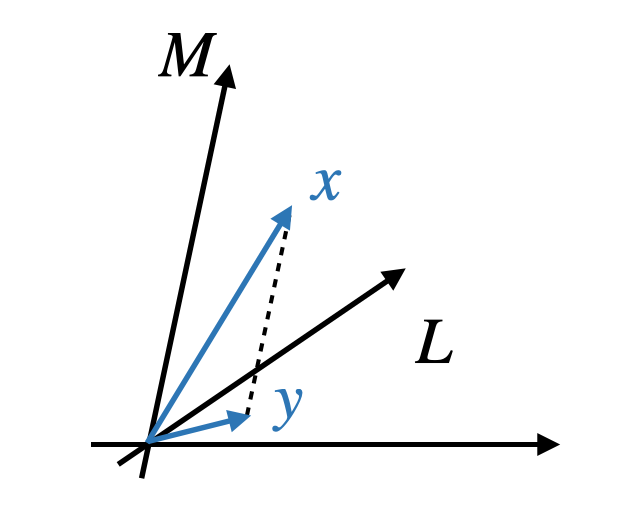
\includegraphics[width=0.2\linewidth]{figs/proj.png}
\end{figure}
\end{definition}

\begin{property}
$R(P_{L,M})=L,\,N(P_{L,M})=M$. 注意 $x-y\in M$.
\end{property}

\begin{definition}[投影矩阵]
投影算子 $P_{L,M}$ 在 $\mathbb C^n$ 的基 $(e_1,\ldots,e_n)$ 下的矩阵称为投影矩阵。
\end{definition}

\begin{lemma}
设 $A\in\mathbb C^{n\times n}$ 是幂等矩阵,即 $A^2=A$,则:
\[N(A)=R(I-A)\]
\end{lemma}
\begin{proof}
任取 $x\in N(A)$,则 $Ax=0$,则 $x=Ax+(I-A)x=(I-A)x\in R(I-A)$,因此 $N(A)\subset R(I-A)$;
任取 $y\in\mathbb C^n$,$A(I-A)y=(A-A^2)y=0$,故 $(I-A)y\in N(A)$,故 $R(I-A)\subset N(A)$;
综上,$N(A)=R(I-A)$.
\end{proof}

\begin{theorem}[投影与幂等]
矩阵 $P$ 为投影矩阵的充要条件是 $P$ 为幂等矩阵,即:
\[
    P_{n\times n}=P_{L,M}\iff P^2=P
\]
\end{theorem}
\begin{proof}
必要性:设 $C^n=L\oplus M$,则对于任意 $x\in\mathbb C^n$,存在唯一的分解 $x=y+z,\,y\in L,\,z\in M$.  于是 $P_{L,M}x=y$. 因此 $P_{L,M}^2x=P_{L,M}y=y=P_{L,M}x$,即 $P_{L,M}$ 是幂等的。

充分性:任意 $x\in\mathbb C^n$ 可分解为 $x=Px+(I-P)x$,根据引理知 $N(P)=R(I-P)$,又 $\mathbb C^n=R(P)\oplus N(P)$,所以这样的分解是唯一的,于是 $P=P_{R(P),N(P)}$.
\end{proof}

\noindent\textbf{计算方法}:取 $L$ 的一组基 $(q_1,\ldots,q_r)$ 和 $M$ 的一组基 $(q_{r+1},\ldots,q_n)$,则任意向量 $x\in\mathbb C^n$ 可表示为:
\[
    x=(q_1,\ldots,q_r,q_{r+1},\ldots,q_n)y=Qy
\]
于是:
\[
    P_{L,M}x=QI_ry=QI_rQ^{-1}x\implies P_{L,M}=QI_rQ^{-1}
\]
其中 $I_r$ 表示前 $r$ 个对角元为 1、其余为 0 的对角矩阵。

\begin{com}
可以看见上面的计算方法涉及到基的选取,但可以证明选取不同的基算出来的 $P_{L,M}$ 都是一样的。
假设另选一组基 $\bar Q_L=(\bar q_1,\ldots,\bar q_r)$ 和 $\bar Q_M=(\bar q_{r+1},\ldots,\bar q_n)$,设 $\bar Q_L=Q_LR_1,\,\bar Q_M=Q_MR_2$,则 $\bar Q=Q\text{diag}(R_1,R_2)$,于是:
\[
    \bar P_{L,M}=\bar Q I_r\bar Q^{-1}=Q\text{diag}(R_1,R_2)I_r\text{diag}(R_1^{-1},R_2^{-1})Q^{-1}=QI_rQ^{-1}=P_{L,M}
\]
可见 $P_{L,M}$ 与基的选取无关。
\end{com}

\begin{definition}[正交投影算子]
设 $L$ 是 $\mathbb C^n$ 的子空间,则沿着 $L^{\perp}$ 到 $L$ 的投影算子 $P_{L,L^{\perp}}$ 为正交投影算子,简记为 $P_L$.
\begin{figure}[H]
    \centering
    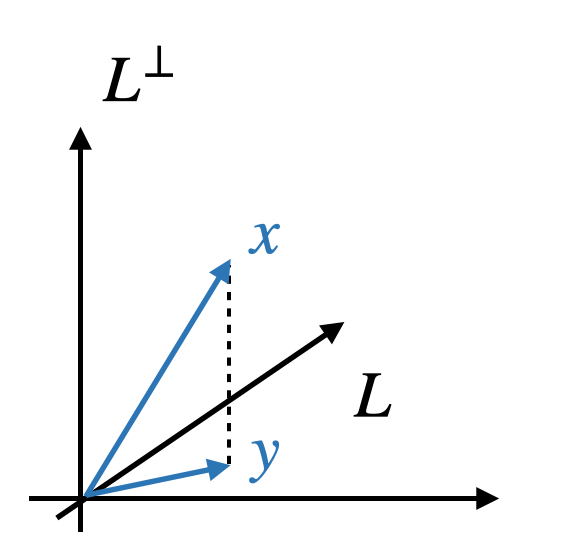
\includegraphics[width=0.2\linewidth]{figs/proj-o.png}
\end{figure}
\end{definition}

\begin{definition}[正交投影矩阵]
正交投影算子 $P_{L}$ 在 $\mathbb C^n$ 的基 $e_1,\ldots,e_n$ 下的矩阵称为正交投影矩阵。
\end{definition}


\begin{theorem}[正交投影与幂等 Hermite]
矩阵 $P$ 为正交投影矩阵的充要条件是 $P$ 为幂等 Hermite 矩阵。
\end{theorem}
\begin{proof}
必要性:若 $P$ 为正交投影矩阵,则根据上一节定理知它是幂等矩阵,于是 $R(I-P)=N(P)$。又 $R(P)\perp N(P)$,所以 $R(P)\perp R(I-P)$,因此对于任意 $x,y\in\mathbb C^n$,有:
\begin{align*}
    x^HP^H(I-P)y=0&\implies P^H(I-P)=0\implies P^H=P^HP\\&\implies P=(P^HP)^H=P^HP=P^H
\end{align*}
即 $P$ 是 Hermite 矩阵。

充分性:若 $P$ 是幂等 Hermite 矩阵,则根据上一节定理知它是投影矩阵 $P_{R(P),N(P)}$.  又由于 $P^H=P$,所以:
\[
    P_{R(P),N(P)}=P_{R(P),N(P^H)}=P_{R(P),R^\perp(P)}
\]
即 $P$ 是正交投影矩阵。
\end{proof}

\noindent\textbf{计算方法}:取 $L$ 的一组基 $X=(x_1,\ldots,x_r)$,$L^{\perp}$ 的一组基 $y=(y_1,\ldots,y_{n-r})$,则 $X^HY=Y^HX=O$.  根据上一节投影矩阵的计算方法知:
\[
    P_L=P_{L,L^\perp}
    =\left[\begin{array}{c:c}X&Y\end{array}\right]\;I_r\;\left[\begin{array}{c:c}X&Y\end{array}\right]^{-1}
    =\left[\begin{array}{c:c}X&O\end{array}\right]\left[\begin{array}{c:c}X&Y\end{array}\right]^{-1}
\]
由于:
\[
    \left[\begin{array}{c:c}X&Y\end{array}\right]^{H}\left[\begin{array}{c:c}X&Y\end{array}\right]=\left[\begin{array}{c}X^H\\\hdashline Y^H\end{array}\right]\left[\begin{array}{c:c}X&Y\end{array}\right]=\left[\begin{array}{c:c}X^HX&O\\\hdashline O&Y^HY\end{array}\right]
\]
于是:
\[
    \left[\begin{array}{c:c}X&Y\end{array}\right]^{-1}=\left[\begin{array}{c:c}(X^HX)^{-1}&O\\\hdashline O&(Y^HY)^{-1}\end{array}\right]\left[\begin{array}{c}X^H\\\hdashline Y^H\end{array}\right]=\left[\begin{array}{c}(X^HX)^{-1}X^H\\\hdashline(Y^HY)^{-1}Y^H\end{array}\right]
\]
因此:
\[
    P_L=\left[\begin{array}{c:c}X&O\end{array}\right]\left[\begin{array}{c:c}X&Y\end{array}\right]^{-1}=\left[\begin{array}{c:c}X&O\end{array}\right]\left[\begin{array}{c}(X^HX)^{-1}X^H\\\hdashline(Y^HY)^{-1}Y^H\end{array}\right]=X(X^HX)^{-1}X^H
\]

\begin{com}
同样的,正交投影矩阵的计算也与选取的基无关。假设有另一组基 $\bar X=(\bar x_1,\ldots,\bar x_r)$,设 $\bar X=XR$,则:
\begin{align*}
    \bar P_L&=\bar X({\bar X}^H\bar X)^{-1}{\bar X}^H=XR(R^HX^HXR)^{-1}R^HX^H\\
    &=XRR^{-1}(X^HX)^{-1}(R^H)^{-1}R^HX^H=X(X^HX)^{-1}X^H=P_L
\end{align*}
可见 $P_L$ 与基的选取无关。
\end{com}

\begin{remark}
由于 $X$ 是列满秩矩阵,根据下一节的内容可知 $X^+=(X^HX)^{-1}X$,所以 $P_L=XX^+$.
\end{remark}


\subsection{广义逆矩阵的存在、性质及构造方法}

\begin{definition}
\label{def:moore-penrose}
设矩阵 $A\in\mathbb C^{m\times n}$,若矩阵 $X\in\mathbb C^{n\times m}$ 满足如下四个 Penrose 方程:
\begin{align*}
    &AXA=A\tag{1}\label{1}\\
    &XAX=X\tag{2}\label{2}\\
    &(AX)^H=AX\tag{3}\label{3}\\
    &(XA)^H=XA\tag{4}\label{4}
\end{align*}
则称 $X$ 为 $A$ 的 Moore-Penrose 逆,记作 $A^+$.
若 $X$ 值满足上述四个方程中的第 $(i),(j),\ldots,(l)$ 个方程,则称 $X$ 为 $A$ 的 $\{i,j,\ldots,l\}$-逆,记作 $A^{(i,j,\ldots,l)}$,其全体记为 $A\{i,j,\ldots,l\}$.

如下为 1-逆的示意图:
\begin{figure}[H]
    \centering
    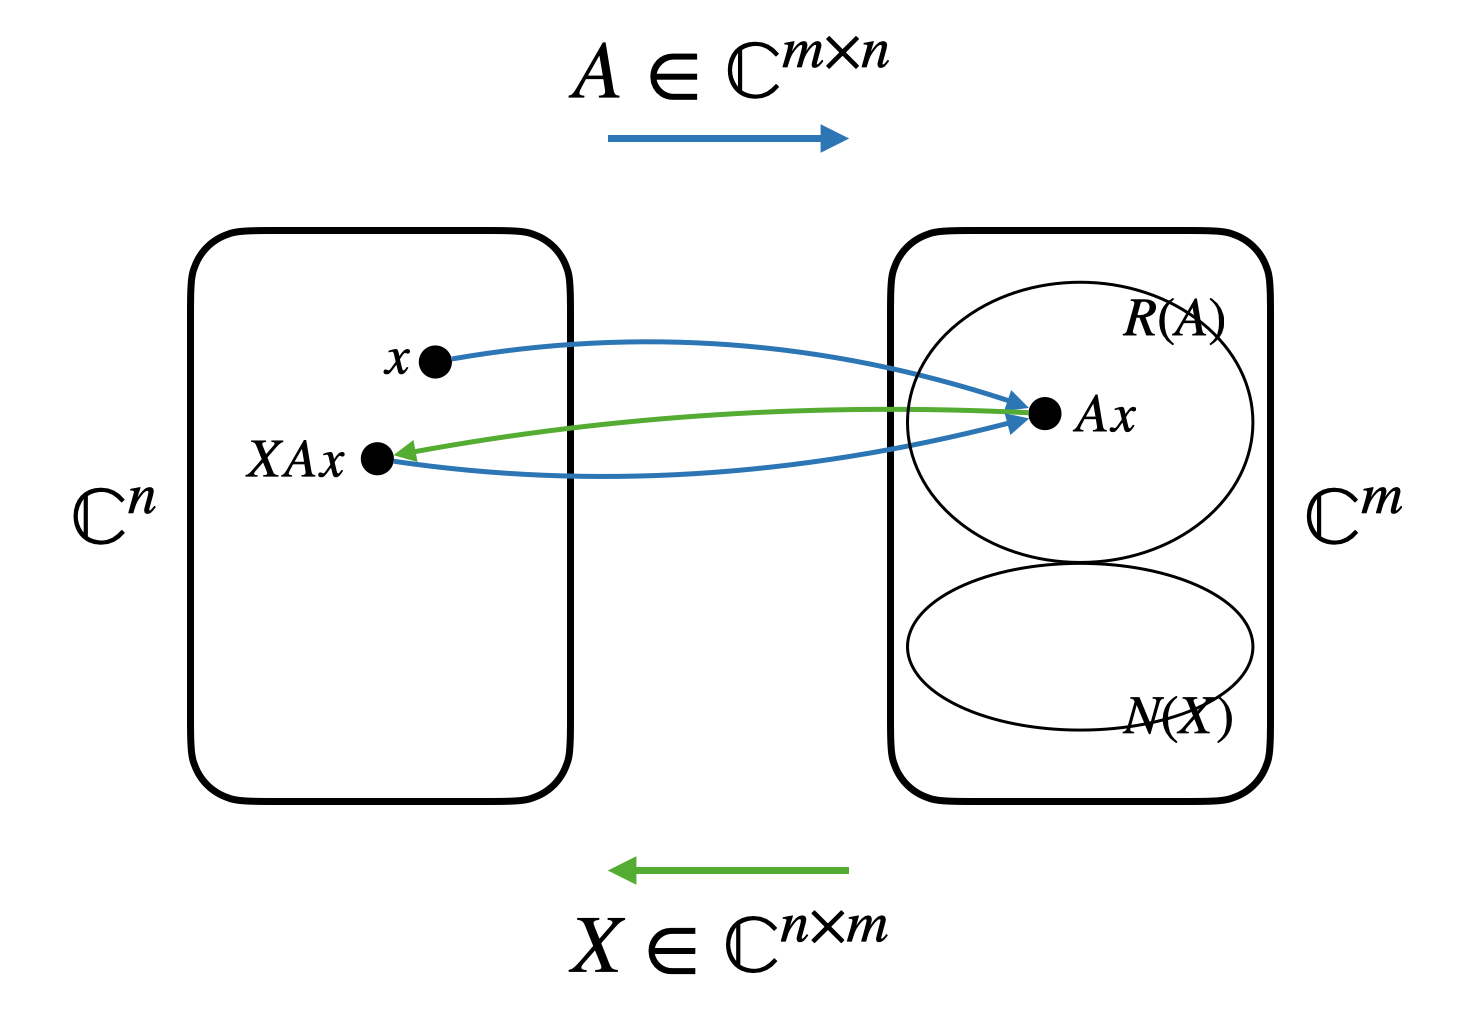
\includegraphics[width=0.5\linewidth]{figs/1inv.png}
\end{figure}
\end{definition}

\begin{theorem}
对任意 $A\in\mathbb C^{m\times n}$,$A^+$ 存在且唯一。
\end{theorem}
\begin{proof}
存在性。对 $A$ 做奇异值分解 $A=U\begin{bmatrix}\Sigma&0\\0&0\end{bmatrix}V^H$,取 $X=V\begin{bmatrix}\Sigma^{-1}&0\\0&0\end{bmatrix}U^H$,可以验证 $X$ 满足 $A^+$ 的四个条件。

唯一性。设 $X,Y$ 均是 $A^+$,则:
\begin{align*}
    Y&=YAY=Y(AY)^H=YY^HA^H=YY^H(AXA)^H\\&=YY^HA^H(AX)^H=Y(AY)^HAX=YAYAX=YAX\\
    X&=XAX=(XA)^HX=A^HX^HX=(AYA)^HX^HX\\&=(YA)^HA^HX^HX=(YA)^H(XA)^HX=(YA)^HXAX=(YA)^HX=YAX
\end{align*}
故 $X=Y$.
\end{proof}

\begin{remark}
上述定理的证明过程也给出了 $A^+$ 的一种基于奇异值分解的计算方法:
\[
    A=U\begin{bmatrix}\Sigma&0\\0&0\end{bmatrix}V^H\implies     A^+=V\begin{bmatrix}\Sigma^{-1}&0\\0&0\end{bmatrix}U^H
\]
\end{remark}

\begin{theorem}
\[
    \lim_{\delta\to0}(\delta^2I+A^HA)^{-1}A^H=A^+
\]
\end{theorem}
\begin{proof}
设 $A=U\begin{bmatrix}\Sigma&0\\0&0\end{bmatrix}V^H$,则 $A^HA=V\begin{bmatrix}\Sigma^2&0\\0&0\end{bmatrix}V^H$,于是:
\[\delta^2I+A^HA=V\begin{bmatrix}\Sigma^2+\delta^2I&0\\0&\delta^2I\end{bmatrix}V^H\]
因此:
\begin{align*}
    (\delta^2I+A^HA)^{-1}A^H&=V\begin{bmatrix}\left[\sigma_i^2+\delta^2\right]_{r\times r}&0\\0&\delta^2I\end{bmatrix}^{-1}V^HA^H\\
    &=V\begin{bmatrix}\left[\dfrac{1}{\sigma_i^2+\delta^2}\right]_{r\times r}&0\\0&\delta^{-2}I\end{bmatrix}(AV)^H\\
    &=V\begin{bmatrix}\left[\dfrac{1}{\sigma_i^2+\delta^2}\right]_{r\times r}&0\\0&\delta^{-2}I\end{bmatrix}\begin{bmatrix}\Sigma&0\\0&0\end{bmatrix}U^H\\
    &=V\begin{bmatrix}\left[\dfrac{\sigma_i}{\sigma_i^2+\delta^2}\right]_{r\times r}&0\\0&0\end{bmatrix}U^H\\
\end{align*}
于是当 $\delta\to0$ 时,
\[
\lim_{\delta\to0}(\delta^2I+A^HA)^{-1}A^H=\lim_{\delta\to0}V\begin{bmatrix}\left[\dfrac{\sigma_i}{\sigma_i^2+\delta^2}\right]_{r\times r}&0\\0&0\end{bmatrix}U^H=V\begin{bmatrix}\Sigma^{-1}&0\\0&0\end{bmatrix}U^H=A^+
\]
\end{proof}

\begin{lemma}
\begin{align*}
    N(A)\supset N(B)&\iff \exists X,A=XB\\
    R(A)\subset R(B)&\iff \exists X,A=BX
\end{align*}
\end{lemma}

\begin{corollary}
\label{cor:rankAB}
\begin{align*}
    &\text{rank}(AB)=\text{rank}(A)\implies \exists X,A=ABX\\
    &\text{rank}(BA)=\text{rank}(A)\implies \exists X,A=XBA
\end{align*}
\end{corollary}
\begin{proof}
由于 $R(AB)\subset R(A)$,且 $\dim R(AB)=\text{rank}(AB)=\text{rank}(A)=\dim R(A)$,故 $R(AB)=R(A)$.  于是 $R(AB)\supset R(A)$,根据引理知 $\exists X,A=ABX$.

类似地,由于 $N(BA)\supset N(A)$,且 $\dim N(BA)=n-\text{rank}(BA)=n-\text{rank}(A)=\dim N(A)$,故 $N(BA)=N(A)$.  于是 $N(BA)\subset N(A)$,根据引理知 $\exists X,A=XBA$.
\end{proof}

\begin{remark}
推论的这两个式子在证明中\textbf{非常常用},即用更复杂的式子表示简单的矩阵,反而有助于证明。
\end{remark}

\begin{theorem}
矩阵 $A\in\mathbb C^{m\times n}$ 有唯一 1-逆的充要条件为 $A$ 是非奇异矩阵,且该 1-逆就是 $A^{-1}$.
\end{theorem}
\begin{proof}
充分性显然,必要性证明如下。设 $Au=0$,$AXA=A$,那么容易验证 $X'=X+u\cdot[1,0,\ldots,0]$ 也满足 $AX'A=A$,由于 1-逆唯一,故 $u=0$,即 $N(A)=\{0\}$.  类似可以证明 $N(A^H)=\{0\}$,于是 $A$ 列满秩且行满秩,故 $A$ 为可逆方阵。
\end{proof}

\begin{property}[1]
$(A^{(1)})^H\in A^{H}\{1\}$.
\end{property}

\begin{property}[2]
$\lambda^+ A^{(1)}\in(\lambda A)\{1\}$. 其中 $\lambda\in\mathbb C,\,\lambda^{+}=\begin{cases}\lambda^{-1},&\lambda\neq 0\\0,&\lambda=0\end{cases}$.
\end{property}

\begin{property}[3]
若 $S$ 和 $T$ 非奇异,则 $T^{-1}A^{(1)}S^{-1}\in(SAT)\{1\}$.
\end{property}

\begin{property}[4]
$\text{rank}(A^{(1)})\geq \text{rank}(A)$.
\end{property}
\begin{proof}
$\text{rank}(A)=\text{rank}(AA^{(1)}A)\leq\text{rank}(A^{(1)})$.
\end{proof}

\begin{property}[5]
$AA^{(1)}$ 和 $A^{(1)}A$ 均为幂等矩阵且与 $A$ 同秩。
\end{property}
\begin{proof}
$\text{rank}(AA^{(1)})\leq\text{rank}(A)=\text{rank}(AA^{(1)}A)\leq\text{rank}(AA^{(1)})$,故 $\text{rank}(AA^{(1)})=\text{rank}(A)$.
\end{proof}

\begin{property}[6]
$R(AA^{(1)})=R(A),\,N(A^{(1)}A)=N(A),\,R((A^{(1)}A)^H)=R(A^H)$.
\end{property}
\begin{proof}
$R(AA^{(1)})\subset R(A)=R(AA^{(1)}A)\subset R(AA^{(1)})$,故 $R(AA^{(1)})=R(A)$.

类似地,$N(A)\subset N(A^{(1)}A)\subset N(AA^{(1)}A)=N(A)$,故 $N(A^{(1)}A)=N(A)$.
\end{proof}

\begin{property}[7]
$A^{(1)}A=I_n\iff \text{rank}(A)=n$,$AA^{(1)}=I_m\iff \text{rank}(A)=m$.
\end{property}
\begin{proof}
根据性质 5,$\text{rank}(A^{(1)}A)=\text{rank}(A)$,因此必要性:$A^{(1)}A=I_n\implies\text{rank}(A^{(1)}A)=n\implies\text{rank}(A)=n$;充分性:$\text{rank}(A)=n\implies \text{rank}(A^{(1)}A)=n$,即 $A^{(1)}A$ 可逆,又 $A^{(1)}A$ 幂等,故为单位阵。另一个类似。证毕。
\end{proof}

\begin{property}[8]
推论 \ref{cor:rankAB} 的进一步阐述,给出了存在的 $X$ 的具体形式:
\begin{gather*}
    AB(AB)^{(1)}A=A\iff\text{rank}(AB)=\text{rank}(A)\\
    B(AB)^{(1)}AB=B\iff\text{rank}(AB)=\text{rank}(B)
\end{gather*}
\end{property}
\begin{proof}
这里只证明第一行,第二行类似可证。

充分性:根据推论 \ref{cor:rankAB},存在 $X$ 使得 $A=ABX$,于是 $AB(AB)^{(1)}A=AB(AB)^{(1)}ABX=ABX=A$.

必要性:$\text{rank}(A)\geq\text{rank}(AB)\geq\text{rank}(AB(AB)^{(1)}A)=\text{rank}(A)$,故 $\text{rank}(AB)=\text{rank}(A)$.
\end{proof}

\begin{theorem}
设 $Y,Z\in A\{1\}$,则 $X=YAZ\in A\{1,2\}$.
\end{theorem}
\begin{proof}
$XAX=YAZAYAZ=YAYAZ=YAZ=X$,故 $X\in A\{2\}$. 又 $AXA=AYAZA=AZA=A$,故 $X\in A\{1\}$. 综上,$X\in A\{1,2\}$.
\end{proof}
\begin{proof}[证明 2(利用通解形式,见下文)]
奇异值分解 $A=U\begin{bmatrix}\Sigma&0\\0&0\end{bmatrix}V^H$,则 $Y,Z$ 可分别写作:
\[
    Y=V\begin{bmatrix}\Sigma&C_1\\D_1&E_1\end{bmatrix}U^H,\quad Z=V\begin{bmatrix}\Sigma&C_2\\D_2&E_2\end{bmatrix}U^H
\]
于是:
\[
    X=YAZ=V\begin{bmatrix}B^{-1}&C_1\\D_1&E_1\end{bmatrix}U^HU\begin{bmatrix}B&0\\0&0\end{bmatrix}V^HV\begin{bmatrix}B^{-1}&C_2\\D_2&E_2\end{bmatrix}U^H=V\begin{bmatrix}B^{-1}&C_2\\D_1&D_1BC_2\end{bmatrix}U^H
\]
这正是 1,2-逆的通解形式,故 $X\in A\{1,2\}$.
\end{proof}

\begin{theorem}
给定矩阵 $A$ 和 $X\in A\{1\}$,则 $X\in A\{1,2\}$ 的充要条件是 $\text{rank}(X)=\text{rank}(A)$.
\end{theorem}
\begin{proof}
充分性。由于 $X\in A\{1\}$,故 $A=AXA$,于是 $\text{rank}(A)=\text{rank}(AXA)\leq\text{rank}(XA)\leq\text{rank}(X)=\text{rank}(A)$,故 $\text{rank}(X)=\text{rank}(XA)$. 根据推论,存在 $Y$ 使得 $X=XAY$,于是 $XAX=XAXAY=XAY=X$,故 $X\in A\{2\}$.

必要性。由于 $A=AXA,\,XAX=X$,于是 $\text{rank}(X)=\text{rank}(XAX)\leq\text{rank}(A)=\text{rank}(AXA)\leq\text{rank}(X)$,故 $\text{rank}(X)=\text{rank}(A)$.
\end{proof}

\begin{lemma}
对任意矩阵 $A$ 均有:
\[
    \text{rank}(A^HA)=\text{rank}(A)=\text{rank}(AA^H)
\]
\end{lemma}
\begin{proof}
由于 $A^HAx=0\implies x^HA^HAx=0\implies Ax=0$,所以 $N(A^HA)\subset N(A)$.  又 $N(A^HA)\supset N(A)$,于是 $N(A^HA)=N(A)$,于是 $\text{rank}(A^HA)=\text{rank}(A)$. 另一个类似。
\end{proof}

\begin{theorem}
设有矩阵 $A$,则:
\begin{align*}
    &Y=(A^HA)^{(1)}A^H\in A\{1,2,3\}\\
    &Z=A^H(AA^H)^{(1)}\in A\{1,2,4\}
\end{align*}
\end{theorem}
\begin{proof}
由于 $\text{rank}(A^HA)=\text{rank}(A)=\text{rank}(AA^H)$,根据 1-逆的性质 8 有:
\[
    A=A(A^HA)^{(1)}A^HA,\quad A^H=A^HA(A^HA)^{(1)}A^H
\]
因此:
\begin{align*}
    &AYA=A(A^HA)^{(1)}A^HA=A&\implies Y\in A\{1\}\\
    &YAY=(A^HA)^{(1)}A^HA(A^HA)^{(1)}A^H=(A^HA)^{(1)}A^H=Y&\implies Y\in A\{2\}
\end{align*}
又存在 $X$ 使得 $A=XA^HA$,故:
\begin{align*}
    AY&=A(A^HA)^{(1)}A^H=(XA^HA)(A^HA)^{(1)}(XA^HA)^H\\
    &=XA^HA(A^HA)^{(1)}A^HAX^H=XA^HAX^H
\end{align*}
是 Hermite 矩阵,于是 $Y\in A\{3\}$.
$Z$ 可类似证明。
\end{proof}

\begin{theorem}
\[
    A^+=A^{(1,4)}AA^{(1,3)}
\]
\end{theorem}
\begin{proof}
设 $X=A^{(1,4)}AA^{(1,3)}$,根据关于 1,2-逆的定理知 $X\in A\{1,2\}$. 另外,
\[
    AX=AA^{(1,4)}AA^{(1,3)}=AA^{(1,3)},\quad XA=A^{(1,4)}AA^{(1,3)}A=A^{(1,4)}A
\]
均是 Hermite 矩阵,从而得到结论。
\end{proof}
\begin{proof}[证明 2(利用通解形式,见下文)]
{\color{red}{TODO}}
\end{proof}

\begin{theorem}
给定矩阵 $A\in\mathbb C^{m\times n}$,有:
\begin{enumerate}
    \item $\text{rank}(A^+)=\text{rank}(A)$.
    \item $(A^+)^+=A$.
    \item $(A^H)^+=(A^+)^H,\,(A^T)^+=(A^+)^T$.
    \item $(A^HA)^+=A^+(A^H)^+,\,(AA^H)^+=(A^H)^+A^+$.
    \item $A^+=(A^HA)^+A^H=A^H(AA^H)^+$.
    \item $R(A^+)=R(A^H),\,N(A^+)=N(A^H)$.
\end{enumerate}
\end{theorem}
\begin{proof}
前 5 条都可以通过定义证明。对于第 6 条,根据 1 可知 $\text{rank}(A^+)=\text{rank}(A)=\text{rank}(A^H)$,根据 5 可知 $R(A^+)\subset R(A^H),\,N(A^+)\supset N(A^H)$,于是 $R(A^+)=R(A^H),\,N(A^+)=N(A^H)$.
\end{proof}

\begin{corollary}
若 $A\in\mathbb C_n^{m\times n}$,即列满秩,则 $A^+=(A^HA)^{-1}A^H$;若 $A\in\mathbb C_m^{m\times n}$,即行满秩,则 $A^+=A^H(AA^H)^{-1}$.
\end{corollary}

\begin{corollary}
若 $\alpha\in\mathbb C^n$,且 $\alpha\neq 0$,则 $\alpha^+=(\alpha^H\alpha)^{-1}\alpha^H$,而 $(\alpha^H)^+=(\alpha^+)^H=\alpha(\alpha^H\alpha)^{-1}$.
\end{corollary}

\vskip 6pt \noindent\textbf{广义逆的通解形式}:
设 $A\in\mathbb C^{m\times n}_r$,则存在 $m$ 阶可逆矩阵(或酉矩阵)$P$ 和 $n$ 阶可逆矩阵(或酉矩阵)$Q$ 使得 $A=P\begin{bmatrix}B&0\\0&0\end{bmatrix}Q$,其中 $B$ 为 $r$ 阶可逆矩阵。那么,各广义逆的通解形式如下表所示:

\begin{table}[H]
    \centering
    \begin{tabular}{ll}
    \toprule
    \textbf{广义逆} & \textbf{通解} \\ \midrule
    $X \in A\{1\}$ & $\exists\ C,D,E,\quad\;X=Q^{-1}\begin{bmatrix}B^{-1}&C\\D&E\end{bmatrix}P^{-1}$ \\
    $X \in A\{1,2\}$ & $\exists\ C,D,\quad X=Q^{-1}\begin{bmatrix}B^{-1}&C\\D&DBC\end{bmatrix}P^{-1}$ \\
    $X \in A\{1,3\}$ & $\exists\ D,E,\quad\;X=Q^{-1}\begin{bmatrix}B^{-1}&0\\D&E\end{bmatrix}P^{-1}$ \\
    $X \in A\{1,4\}$ & $\exists\ C,E,\quad\;X=Q^{-1}\begin{bmatrix}B^{-1}&C\\0&E\end{bmatrix}P^{-1}$ \\
    $X \in A\{1,2,3\}$ & $\exists\ D,\quad\;X=Q^{-1}\begin{bmatrix}B^{-1}&0\\D&0\end{bmatrix}P^{-1}$ \\
    $X \in A\{1,2,4\}$ & $\exists\ C,\quad\;X=Q^{-1}\begin{bmatrix}B^{-1}&C\\0&0\end{bmatrix}P^{-1}$ \\
    $X \in A\{1,3,4\}$ & $\exists\ E,\quad\;X=Q^{-1}\begin{bmatrix}B^{-1}&0\\0&E\end{bmatrix}P^{-1}$ \\
    $X \in A\{1,2,3,4\}$ & $X=Q^{-1}\begin{bmatrix}B^{-1}&0\\0&0\end{bmatrix}P^{-1}$ \\ \bottomrule
    \end{tabular}
\end{table}

% |       广义逆        |                             通解                             |
% | :-----------------: | :----------------------------------------------------------: |
% |    $X\in A\{1\}$    | $\exists\ C,D,E,\quad\;X=Q^{-1}\begin{bmatrix}B^{-1}&C\\D&E\end{bmatrix}P^{-1}$ |
% |   $X\in A\{1,2\}$   | $\exists\ C,D,\quad X=Q^{-1}\begin{bmatrix}B^{-1}&C\\D&DBC\end{bmatrix}P^{-1}$ |
% |   $X\in A\{1,3\}$   | $\exists\ D,E,\quad\;X=Q^{-1}\begin{bmatrix}B^{-1}&0\\D&E\end{bmatrix}P^{-1}$ |
% |   $X\in A\{1,4\}$   | $\exists\ C,E,\quad\;X=Q^{-1}\begin{bmatrix}B^{-1}&C\\0&E\end{bmatrix}P^{-1}$ |
% |  $X\in A\{1,2,3\}$  | $\exists\ D,\quad\;X=Q^{-1}\begin{bmatrix}B^{-1}&0\\D&0\end{bmatrix}P^{-1}$ |
% |  $X\in A\{1,2,4\}$  | $\exists\ C,\quad\;X=Q^{-1}\begin{bmatrix}B^{-1}&C\\0&0\end{bmatrix}P^{-1}$ |
% |  $X\in A\{1,3,4\}$  | $\exists\ E,\quad\;X=Q^{-1}\begin{bmatrix}B^{-1}&0\\0&E\end{bmatrix}P^{-1}$ |
% | $X\in A\{1,2,3,4\}$ |  $X=Q^{-1}\begin{bmatrix}B^{-1}&0\\0&0\end{bmatrix}P^{-1}$   |

% 如果 $P,Q$ 是酉矩阵,则 $Q^{-1},P^{-1}$ 写为 $Q^H,P^H$ 即可。
\begin{remark}
与通解形式相对应,称定义 \ref{def:moore-penrose} 中给出的广义逆的定义为方程形式。
做证明时,有时使用方程形式不容易想到思路,而使用通解只需要无脑计算即可。
\end{remark}
\begin{remark}
应用奇异值分解可以使得 $A=U\begin{bmatrix}\Sigma&0\\0&0\end{bmatrix}V^H$,这是上面的特殊情形,因此\textbf{做证明题时直接奇异值分解}就行了。
但是做计算题时,奇异值分解比较麻烦,所以我们不必追求让 $B$ 成为对角矩阵,只需要使得 $B$ 可逆即可。可以通过如下方式计算 $P,Q,B$:
\[
    \begin{bmatrix}A&I_m\\I_n&0\end{bmatrix}\xrightarrow[\text{列变换}]{\text{行变换}}\begin{bmatrix}\begin{bmatrix}B&0\\0&0\end{bmatrix}&P\\Q&0\end{bmatrix}
\]
也可以通过 QR 分解做:首先使用列置换矩阵 $P$ 使得 $AP$ 前 $r$ 列线性无关,则对 $AP$ 做 QR 分解得 $AP=Q_1\begin{bmatrix}R_1&G\\0&0\end{bmatrix}$,其中 $R_1$ 为上三角矩阵。再对 $\begin{bmatrix}R_1^H&0\\G^H&0\end{bmatrix}$ 做 QR 分解得 $\begin{bmatrix}R_1^H&0\\G^H&0\end{bmatrix}=Q_2\begin{bmatrix}R_2&0\\0&0\end{bmatrix}$,其中 $R_2$ 为上三角矩阵。于是:
\[
    AP=Q_1\begin{bmatrix}R_2^H&0\\0&0\end{bmatrix}Q_2^H\implies A=Q_1\begin{bmatrix}R_2^H&0\\0&0\end{bmatrix}Q_2^HP^T
\]
这样得到的 $B$ 是一个下三角矩阵。
\end{remark}

\begin{definition}[广义逆的等价定义]
设 $A\in\mathbb C^{m\times n}$,若矩阵 $X\in\mathbb C^{n\times m}$ 满足 $AX=P_{R(A)},\,XA=P_{R(X)}$,其中 $P_L$ 是空间 $L$ 上的正交投影矩阵,则称 $X$ 为 $A$ 的 Moore 广义逆矩阵。
\end{definition}

\begin{theorem}
Moore 广义逆矩阵和 Penrose 广义逆矩阵是等价的。
\end{theorem}


\subsection{广义逆矩阵的计算方法}

\begin{theorem}[利用 Hermite 标准形计算 1-逆和 1,2-逆]
设 $A\in\mathbb C_r^{m\times n}$,又设 $Q\in\mathbb C_m^{m\times m}$ 和 $P\in\mathbb C_n^{n\times n}$ 使得
\[
    QAP=\begin{bmatrix}I_r&K\\0&0\end{bmatrix}
\]
成立($P$ 可以只是一个列置换矩阵),则对任意 $L\in\mathbb C^{(n-r)\times (m-r)}$,$n\times m$ 矩阵
\[
    X=P\begin{bmatrix}I_r&0\\0&L\end{bmatrix}Q
\]
是 $A$ 的 1-逆,若令 $L=0$ 则 $X$ 是 $A$ 的 1,2-逆。
\end{theorem}

\begin{remark}
理论基础显然是上一节的 1-逆和 1,2-逆的通解形式,不过这里不要求 $K=0$,相应代价就是通解中的 $C,D$ 这里必须是零,也就是说得到的是一种特解。
\end{remark}

\begin{theorem}[满秩分解求广义逆矩阵]
设 $A\in\mathbb C_r^{m\times n}$ 的满秩分解为 $A=FG$,则:
\begin{enumerate}
    \item $G^{(i)}F^{(1)}\in A\{i\},\,i=1,2,4$.
    \item $G^{(1)}F^{(i)}\in A\{i\},\,i=1,2,3$.
    \item $G^{(1)}F^{+}\in A\{1,2,3\}$,$G^{+}F^{(1)}\in A\{1,2,4\}$.
    \item $A^+=G^+F^{(1,3)}=G^{(1,4)}F^+$.
    \item $A^+=G^+F^+=G^H(GG^H)^{-1}(F^HF)^{-1}F^H$.
\end{enumerate}
\end{theorem}

\begin{remark}
由于 $F$ 列满秩、$G$ 行满秩,根据上一节 1-逆的性质 7,有 $F^{(1)}F=GG^{(1)}=I_r$.  利用这一点,由定义即可验证 1 与 2。
3 和 4 可由 1 和 2 得到。5 利用了上一节关于行满秩与列满秩的矩阵的 $A^+$ 公式。
\end{remark}

\begin{theorem}[Zlobec 公式计算 $A^+$]
\[
    A^+=A^H(A^HAA^H)^{(1)}A^H
\]
\end{theorem}
\begin{proof}[证明(利用通解形式)]
设 $A=U\begin{bmatrix}\Sigma&0\\0&0\end{bmatrix}V^H$,则:
\[
    A^HAA^H=V\begin{bmatrix}\Sigma&0\\0&0\end{bmatrix}U^HU\begin{bmatrix}\Sigma&0\\0&0\end{bmatrix}V^HV\begin{bmatrix}\Sigma&0\\0&0\end{bmatrix}U^H=V\begin{bmatrix}\Sigma^3&0\\0&0\end{bmatrix}U^H
\]
于是:
\[
    (A^HAA^H)^{(1)}=U\begin{bmatrix}\Sigma^{-3}&C\\D&E\end{bmatrix}V^H
\]
因此:
\[
    A^H(A^HAA^H)^{(1)}A^H=V\begin{bmatrix}\Sigma&0\\0&0\end{bmatrix}U^HU\begin{bmatrix}\Sigma^{-3}&C\\D&E\end{bmatrix}V^HV\begin{bmatrix}\Sigma&0\\0&0\end{bmatrix}U^H=V\begin{bmatrix}\Sigma^{-1}&0\\0&0\end{bmatrix}U^H
\]
这就是 $A^+$ 的通解形式。
\end{proof}

如果用方程形式去证明,需要一些引理的帮助,显得非常麻烦,这里不做叙述。不过这些引理中有一些值得注意,写在下面。

\begin{theorem}
设 $A\in\mathbb C_r^{m\times n},\,U\in\mathbb C^{n\times p},\,V\in\mathbb C^{q\times m}$,则
\[
    U(VAU)^{(1)}V\in A\{1\}\iff \text{rank}(VAU)=\text{rank}(A)
\]
\end{theorem}
\begin{remark}
这个定理是 1-逆的性质 8 的扩展。回顾性质 8(做了变量替换):
\begin{align*}
    &AU(AU)^{(1)}A=A\iff\text{rank}(AU)=\text{rank}(A)\\
    &A(VA)^{(1)}VA=A\iff\text{rank}(VA)=\text{rank}(A)
\end{align*}
第一条是在 $A$ 的右边乘上 $U$,第二条是在 $A$ 的左边乘上 $V$,而这个定理左右同时乘了 $V$ 和 $U$.
\end{remark}
\begin{proof}
充分性。由 $\text{rank}(VAU)=\text{rank}(A)$ 知 $R(VAU)=R(AU)=R(A),\,N(VAU)=N(VA)=N(A)$. 故存在 $X,Y$ 使得 $A=AUX=YVA$,于是 $AU(VAU)^{(1)}VA=YVAU(VAU)^{(1)}VAUX=YVAUX=YVA=A$.

必要性:{\color{red}{???TODO}}
\end{proof}

\begin{theorem}
对任意矩阵 $A$,满足 $X\in A\{1,2\}$ 和 $R(X)=R(A^H),\,N(X)=N(A^H)$ 的唯一矩阵为 $A^+$.
\end{theorem}

\begin{theorem}[Greville 公式计算 $A^+$]
Greville 公式是计算 $A^+$ 的**增量**公式。
设 $A\in\mathbb C^{m\times n}$,记 $a_k$ 为 $A$ 的第 $k$ 列,$A_k$ 为 $A$ 的前 $k$ 列构成的子矩阵;又记:
\[
    d_k=A^+_{k-1}a_k,\quad c_k=a_k-A_{k-1}d_k
\]
则:
\[
    A^+_k=\begin{bmatrix}A^+_{k-1}-d_kb_k^H\\b_k^H\end{bmatrix},\quad\text{where}\quad b_k^H=\begin{cases}c_k^+,&c_k\neq 0\\(1+d_k^Hd_k)^{-1}d_k^HA^+_{k-1},&c_k=0\end{cases}
\]
\end{theorem}


\subsection{广义逆矩阵与线性方程组求解}

对于方程组 $Ax=b$,如果 $A$ 非奇异,则 $x=A^{-1}b$ 是唯一解。而在其他情况下,我们希望得到类似的结果。
\begin{itemize}
    \item 如果方程组相容,且其解有无数多个,我们希望求\textbf{极小范数解},即 $\min_{Ax=b}\Vert x\Vert$;
    \item 如果方程组不相容,即无解,那么我们希望求矛盾方程组的\textbf{最小二乘解},即 $\min \Vert Ax-b\Vert$;
    \item 一般而言,最小二乘解也不唯一,因此我们希望求\textbf{极小范数最小二乘解},即 $\min_{\min\Vert Ax-b\Vert}\Vert x\Vert$.
\end{itemize}
\begin{com}
本节所用范数均为 2 范数。
\end{com}

\begin{theorem}[线性方程组的相容性、通解与 1-逆]
\label{thm:compatible}
设 $A\in\mathbb C^{m\times n},\,B\in\mathbb C^{p\times q},\,D\in\mathbb C^{m\times q}$,则矩阵方程 $AXB=D$ 相容的充要条件是:
\[
    AA^{(1)}DB^{(1)}B=D
\]
当方程相容时,通解为:
\[
    X=A^{(1)}DB^{(1)}+Y-A^{(1)}AYBB^{(1)}
\]
其中 $Y\in\mathbb C^{n\times p}$ 为任意矩阵。
\end{theorem}
\begin{proof}
充分性,取 $X=A^{(1)}DB^{(1)}$ 即可;必要性,若 $AXB=D$ 有解,则 $D=AXB=AA^{(1)}AXBB^{(1)}B=AA^{(1)}DB^{(1)}B$.

对于通解,首先显然 $X=A^{(1)}DB^{(1)}+Y-A^{(1)}AYBB^{(1)}$ 是方程的解;其次,若 $X$ 是方程的解,则取 $Y=X$ 即可写作通解形式。
\end{proof}

\begin{corollary}
设 $A\in\mathbb C^{m\times n}$,取 $A^{(1)}\in A\{1\}$,则:
\[
    A\{1\}=\{A^{(1)}+Z-A^{(1)}AZAA^{(1)}\mid Z\in\mathbb C^{n\times m}\}
\]
\end{corollary}
\begin{proof}
任意 $X\in A\{1\}$ 满足矩阵方程 $AXA=A$,代入上述定理的通解形式得:
\begin{align*}
    X&=A^{(1)}AA^{(1)}+Y-A^{(1)}AYAA^{(1)}\\
    &=A^{(1)}AA^{(1)}+A^{(1)}+Z-A^{(1)}A(A^{(1)}+Z)AA^{(1)}&Y=A^{(1)}+Z\\
    &=A^{(1)}+Z+A^{(1)}AA^{(1)}-A^{(1)}AA^{(1)}AA^{(1)}-A^{(1)}AZAA^{(1)}\\
    &=A^{(1)}+Z-A^{(1)}AZAA^{(1)}
\end{align*}
\end{proof}

\begin{theorem}
\label{thm:compatible2}
线性方程组 $Ax=b$ 相容的充要条件是:
\[
    AA^{(1)}b=b
\]
通解为:
\[
    x=A^{(1)}b+(I-A^{(1)}A)y
\]
其中 $y\in\mathbb C^{n}$ 为任意向量。
\end{theorem}
\begin{proof}
在定理 \ref{thm:compatible} 中取 $X=x,\,B=I,\,D=b$ 即可。
\end{proof}

定理 \ref{thm:compatible2} 是给定 $A^{(1)}$ 后求解方程的解,反过来,利用方程的解也可以给出 $A^{(1)}$.

\begin{theorem}
若对于任意满足 $Ax=b$ 相容的 $b$,$x=Xb$ 都是解,则 $X\in A\{1\}$.
\end{theorem}
\begin{proof}
考虑 $Ax=a_i$,其中 $a_i$ 为 $A$ 的列,由于 $x=Xa_i$ 是方程的解,所以 $AXa_i=a_i$,于是 $AXA=A$,故 $X\in A\{1\}$.
\end{proof}

\begin{lemma}[极小范数解]
相容方程组 $Ax=b$ 的极小范数解唯一,且这个唯一解在 $R(A^H)$ 中。
\end{lemma}
\begin{proof}
由于 $R(A^H)=N(A)^\perp$,所以设 $x=y+z$,其中 $y=P_{R(A^H)}x\in R(A^H),\,z=P_{N(A)}x\in N(A)$,于是:
\[
    \Vert x\Vert^2=\Vert y+z\Vert^2=\Vert y\Vert^2+\Vert z\Vert^2\geq \Vert y\Vert^2
\]
由于 $Az=0\implies Ay=b$,即 $y$ 也是方程的解,所以为了让 $x$ 是极小范数解,只能是 $z=0$,因此 $x=y\in R(A^H)$.

唯一性。设 $x'\in R(A^H)$ 且 $Ax'=b$,则 $A(x-x')=0$,即 $x-x'\in N(A)=R^{\perp}(A^H)$.  又 $x-x'\in R(A^H)$,故 $x-x'=0$.
\end{proof}

\begin{lemma}
集合 $A\{1,4\}$ 由矩阵方程 $XA=A^{(1,4)}A$ 的所有解组成,其中 $A^{(1,4)}\in A\{1,4\}$.
\end{lemma}
\begin{proof}
$AXA=AA^{(1,4)}A=A$,所以 $X\in A\{1\}$;$(XA)^H=(A^{(1,4)}A)^H=A^{(1,4)}A=XA$,所以 $X\in A\{4\}$.  综上 $X\in A\{1,4\}$.

另一方面,若 $X\in A\{1,4\}$,则
\begin{align*}
    A^{(1,4)}A&=A^{(1,4)}AXA=(A^{(1,4)}A)^H(XA)^H=A^H(A^{(1,4)})^HA^HX^H\\
    &=(AA^{(1,4)}A)^HX^H=A^HX^H=XA
\end{align*}
即 $X$ 是方程的解。
\end{proof}

\begin{remark}
该定理说明尽管 $A^{(1,4)}$ 不唯一,但是 $A^{(1,4)}A$ 唯一。
\end{remark}

\begin{corollary}
$A^{(1,4)}A=P_{R(A^H)}$.
\end{corollary}

\begin{theorem}
设 $A\in\mathbb C^{m\times n},\,A^{(1,4)}\in A\{1,4\}$,则:
\[
    A\{1,4\}=\{A^{(1,4)}+Z(I-AA^{(1,4)})\mid Z\in\mathbb C^{n\times m}\}
\]
\end{theorem}
\begin{proof}
根据引理,任意 $X\in A\{1,4\}$ 满足方程 $XA=A^{(1,4)}A$,代入通解形式得:
\begin{align*}
    X&=A^{(1,4)}AA^{(1,4)}+Y-YAA^{(1,4)}\\
    &=A^{(1,4)}AA^{(1,4)}+A^{(1,4)}+Z-(A^{(1,4)}+Z)AA^{(1,4)}&Y=A^{(1,4)}+Z\\
    &=A^{(1,4)}+Z+A^{(1,4)}AA^{(1,4)}-(A^{(1,4)}+Z)AA^{(1,4)}\\
    &=A^{(1,4)}+Z(I-AA^{(1,4)})
\end{align*}
\end{proof}

\begin{theorem}[相容方程组的极小范数解与 1,4-逆]
设 $Ax=b$ 相容,则 $x=A^{(1,4)}b$ 为极小范数解;反之,若对于任意 $b\in R(A)$,$x=Xb$ 都是极小范数解,则 $X\in A\{1,4\}$.
\end{theorem}
\begin{proof}
由第一节定理知 $x=A^{(1,4)}b$ 一定是解。设 $Au=b$,则 $x=A^{(1,4)}b=A^{(1,4)}Au=(A^{(1,4)}A)^Hu=A^H(A^{(1,4)})^Hu\in R(A^H)$,于是根据本节引理知 $x$ 为唯一极小范数解。

反之,考虑 $Ax=a_i$,由于 $x=Xa_i$ 是方程的极小范数解,所以 $Xa_i=A^{(1,4)}a_i$,故 $XA=A^{(1,4)}A$,根据引理知 $X\in A\{1,4\}$.
\end{proof}

\begin{lemma}
集合 $A\{1,3\}$ 由矩阵方程 $AX=AA^{(1,3)}$ 的所有解组成,其中 $A^{(1,3)}\in A\{1,3\}$.
\end{lemma}
\begin{proof}
$AXA=AA^{(1,3)}A=A$,故 $X\in A\{1\}$;$(AX)^H=(AA^{(1,3)})^H=AA^{(1,3)}=AX$,故 $X\in A\{3\}$. 综上 $X\in A\{1,3\}$.

另一方面,若 $X\in A\{1,3\}$,则:
\begin{align*}
    AA^{(1,3)}&=AXAA^{(1,3)}=(AX)^H(AA^{(1,3)})^H=X^HA^H(A^{(1,3)})^HA^H\\
    &=X^H(AA^{(1,3)}A)^H=X^HA^H=AX
\end{align*}
即 $X$ 是方程的解。
\end{proof}

\begin{remark}
该定理说明尽管 $A^{(1,3)}$ 不唯一,但是 $AA^{(1,3)}$ 唯一。
\end{remark}

\begin{corollary}
$AA^{(1,3)}=P_{R(A)}$.
\end{corollary}

\begin{theorem}
设 $A\in\mathbb C^{m\times n},\,A^{(1,3)}\in A\{1,3\}$,则:
\[
    A\{1,3\}=\{A^{(1,3)}+(I-A^{(1,3)}A)Z\mid Z\in\mathbb C^{n\times m}\}
\]
\end{theorem}
\begin{proof}
根据引理,任意 $X\in A\{1,3\}$ 满足方程 $AX=AA^{(1,3)}$,代入通解形式得:
\begin{align*}
    X&=A^{(1,3)}AA^{(1,3)}+Y-A^{(1,3)}AY\\
    &=A^{(1,3)}AA^{(1,3)}+A^{(1,3)}+Z-A^{(1,3)}A(A^{(1,3)}+Z)&Y=A^{(1,3)}+Z\\
    &=A^{(1,3)}+Z+A^{(1,3)}AA^{(1,3)}-A^{(1,3)}A(A^{(1,3)}+Z)\\
    &=A^{(1,3)}+(I-A^{(1,3)}A)Z
\end{align*}
\end{proof}

\begin{theorem}[矛盾方程组的最小二乘解与 1,3-逆]
设有方程 $Ax=b$,则 $x=A^{(1,3)}b$ 为最小二乘解;反之,若对于任意 $b$,$x=Xb$ 都是最小二乘解,则 $X\in A\{1,3\}$.
\end{theorem}

\begin{theorem}[法方程]
$x$ 是方程组 $Ax=b$ 的最小二乘解的充要条件为:
\[
    A^HAx=A^Hb
\]
\end{theorem}

\begin{theorem}[矛盾方程组的极小范数最小二乘解与 $A^+$]
$x=A^+b$ 是方程组 $Ax=b$ 的唯一极小范数最小二乘解。反之,若对所有 $b$,$x=Xb$ 都是方程 $Ax=b$ 的极小范数最小二乘解,则 $X=A^+$.
\end{theorem}

\begin{theorem}
若矩阵方程 $AXB=D$ 不相容,则其极小范数最小二乘解,即满足 $\min_{\min \Vert AXB-D\Vert}\Vert X\Vert$ 的唯一解为 $X=A^+DB^+$.
\end{theorem}
\begin{proof}
方程两边同时行拉直:
\[
    \overline{\text{vec}}(AXB)=\overline{\text{vec}}(D)\implies (A\otimes B^T)\overline{\text{vec}}(X)=\overline{\text{vec}}(D)
\]
其极小范数最小二乘解为:
\[
    \overline{\text{vec}}(X)=(A\otimes B^T)^+\overline{\text{vec}}(D)=(A^+\otimes (B^T)^+)\overline{\text{vec}}(D)=(A^+\otimes (B^+)^T)\overline{\text{vec}}(D)
\]
于是反过来应用拉直算子得 $X=A^+DB^+$.
\end{proof}

\begin{com}
上述过程应用了 $(A\otimes B)^+=A^+\otimes B^+$ 的结论,该结论可以通过定义验证。
\end{com}


\vskip 6pt \noindent\textbf{小结}:对于 $Ax=b$,有:
\begin{itemize}
    \item $Ax=b$ 相容的充要条件是 $AA^{(1)}b=b$
    \item 若 $Ax=b$ 相容,则通解为 $x=A^{(1)}b+(I-A^{(1)}A)y$
    \item 若 $Ax=b$ 相容,则极小范数解为 $x=A^{(1,4)}b$
    \item 若 $Ax=b$ 不相容,则最小二乘解为 $x=A^{(1,3)}b$
    \item 若 $Ax=b$ 不相容,则极小范数最小二乘解为 $x=A^+b$
\end{itemize}

对于 $AXB=D$,有:
\begin{itemize}
    \item $AXB=D$ 相容的充要条件是 $AA^{(1)}DB^{(1)}B=D$
    \item 若 $AXB=D$ 相容,则通解为 $X=A^{(1)}DB^{(1)}+Y-A^{(1)}AYBB^{(1)}$
    \item 若 $AXB=D$ 不相容,则极小范数最小二乘解为 $X=A^+DB^+$
\end{itemize}

\vskip 6pt \noindent\textbf{广义逆的集合表示}

\begin{itemize}
    \item $A\{1\}=\{X\mid AXA=A\}=\{A^{(1)}+Z-A^{(1)}AZAA^{(1)}\mid Z\in\mathbb C^{n\times m}\}$
    \item $A\{1,3\}=\{X\mid AX=AA^{(1,3)}\}=\{A^{(1,3)}+(I-A^{(1,3)}A)Z\mid Z\in\mathbb C^{n\times m}\}$
    \item $A\{1,4\}=\{X\mid XA=A^{(1,4)}A\}=\{A^{(1,4)}+Z(I-AA^{(1,4)})\mid Z\in\mathbb C^{n\times m}\}$
    \item $A\{1,2\}=\{X\mid \text{rank}(X)=\text{rank}(A),\,X\in A\{1\}\}$
\end{itemize}
 \pagebreak

\nocite{*}
\bibliographystyle{unsrt}
\bibliography{references}

% \end{sloppypar}
\end{document}
